% uWaterloo Thesis Template for LaTeX 
% Last Updated June 14, 2017 by Stephen Carr, IST Client Services
% FOR ASSISTANCE, please send mail to rt-IST-CSmathsci@ist.uwaterloo.ca

% Effective October 2006, the University of Waterloo 
% requires electronic thesis submission. See the uWaterloo thesis regulations at
% https://uwaterloo.ca/graduate-studies/thesis.

% DON'T FORGET TO ADD YOUR OWN NAME AND TITLE in the "hyperref" package
% configuration below. THIS INFORMATION GETS EMBEDDED IN THE PDF FINAL PDF DOCUMENT.
% You can view the information if you view Properties of the PDF document.

% Many faculties/departments also require one or more printed
% copies. This template attempts to satisfy both types of output. 
% It is based on the standard "book" document class which provides all necessary 
% sectioning structures and allows multi-part theses.

% DISCLAIMER
% To the best of our knowledge, this template satisfies the current uWaterloo requirements.
% However, it is your responsibility to assure that you have met all 
% requirements of the University and your particular department.
% Many thanks for the feedback from many graduates that assisted the development of this template.

% -----------------------------------------------------------------------

% By default, output is produced that is geared toward generating a PDF 
% version optimized for viewing on an electronic display, including 
% hyperlinks within the PDF.
 
% E.g. to process a thesis called "mythesis.tex" based on this template, run:

% pdflatex mythesis	-- first pass of the pdflatex processor
% bibtex mythesis	-- generates bibliography from .bib data file(s)
% makeindex         -- should be run only if an index is used 
% pdflatex mythesis	-- fixes numbering in cross-references, bibliographic references, glossaries, index, etc.
% pdflatex mythesis	-- fixes numbering in cross-references, bibliographic references, glossaries, index, etc.

% If you use the recommended LaTeX editor, Texmaker, you would open the mythesis.tex
% file, then click the PDFLaTeX button. Then run BibTeX (under the Tools menu).
% Then click the PDFLaTeX button two more times. If you have an index as well,
% you'll need to run MakeIndex from the Tools menu as well, before running pdflatex
% the last two times.

% N.B. The "pdftex" program allows graphics in the following formats to be
% included with the "\includegraphics" command: PNG, PDF, JPEG, TIFF
% Tip 1: Generate your figures and photos in the size you want them to appear
% in your thesis, rather than scaling them with \includegraphics options.
% Tip 2: Any drawings you do should be in scalable vector graphic formats:
% SVG, PNG, WMF, EPS and then converted to PNG or PDF, so they are scalable in
% the final PDF as well.
% Tip 3: Photographs should be cropped and compressed so as not to be too large.

% To create a PDF output that is optimized for double-sided printing: 
%
% 1) comment-out the \documentclass statement in the preamble below, and
% un-comment the second \documentclass line.
%
% 2) change the value assigned below to the boolean variable
% "PrintVersion" from "false" to "true".

% --------------------- Start of Document Preamble -----------------------

% Specify the document class, default style attributes, and page dimensions
% For hyperlinked PDF, suitable for viewing on a computer, use this:
\documentclass[letterpaper,12pt,titlepage,oneside,final]{book}
 
% For PDF, suitable for double-sided printing, change the PrintVersion variable below
% to "true" and use this \documentclass line instead of the one above:
%\documentclass[letterpaper,12pt,titlepage,openright,twoside,final]{book}

% Some LaTeX commands I define for my own nomenclature.
% If you have to, it's better to change nomenclature once here than in a 
% million places throughout your thesis!
\newcommand{\package}[1]{\textbf{#1}} % package names in bold text
\newcommand{\cmmd}[1]{\textbackslash\texttt{#1}} % command name in tt font 
\newcommand{\href}[1]{#1} % does nothing, but defines the command so the
\newcommand{\imgsrc}[1]{\caption*{\scriptsize{Source: #1}}}

% print-optimized version will ignore \href tags (redefined by hyperref pkg).
%\newcommand{\texorpdfstring}[2]{#1} % does nothing, but defines the command
% Anything defined here may be redefined by packages added below...

% This package allows if-then-else control structures.
\usepackage{ifthen}
\newboolean{PrintVersion}
\setboolean{PrintVersion}{false} 
% CHANGE THIS VALUE TO "true" as necessary, to improve printed results for hard copies
% by overriding some options of the hyperref package below.

%\usepackage{nomencl} % For a nomenclature (optional; available from ctan.org)
\usepackage{amsmath,amssymb,amstext} % Lots of math symbols and environments
\usepackage[pdftex]{graphicx} % For including graphics N.B. pdftex graphics driver 
\usepackage{natbib} % For better bibliography formatting
\usepackage[dvipsnames]{xcolor} % Additional colors
\usepackage{multirow}
\usepackage{bm}
\usepackage{todonotes}
\usepackage{caption}
\usepackage[hyphens]{url}

% Hyperlinks make it very easy to navigate an electronic document.
% In addition, this is where you should specify the thesis title
% and author as they appear in the properties of the PDF document.
% Use the "hyperref" package 
% N.B. HYPERREF MUST BE THE LAST PACKAGE LOADED; ADD ADDITIONAL PKGS ABOVE
\usepackage[pdftex,pagebackref=false]{hyperref} % with basic options
		% N.B. pagebackref=true provides links back from the References to the body text. This can cause trouble for printing.
\hypersetup{
    plainpages=false,       % needed if Roman numbers in frontpages
    unicode=false,          % non-Latin characters in Acrobat’s bookmarks
    pdftoolbar=true,        % show Acrobat’s toolbar?
    pdfmenubar=true,        % show Acrobat’s menu?
    pdffitwindow=false,     % window fit to page when opened
    pdfstartview={FitH},    % fits the width of the page to the window
    pdftitle={Disentangled Latent Representation Learning for Stylistic Variation in Neural Language Models},    % title: CHANGE THIS TEXT!
    pdfauthor={Vineet John},    % author: CHANGE THIS TEXT! and uncomment this line
    pdfsubject={Natural Language Processing},  % subject: CHANGE THIS TEXT! and uncomment this line
   	pdfkeywords={nlp} {neural-networks} {style-transfer}, % list of keywords, and uncomment this line if desired
    pdfnewwindow=true,      % links in new window
    colorlinks=true,        % false: boxed links; true: colored links
    linkcolor=blue,         % color of internal links
    citecolor=red,        % color of links to bibliography
    filecolor=magenta,      % color of file links
    urlcolor=cyan           % color of external links
}
\ifthenelse{\boolean{PrintVersion}}{   % for improved print quality, change some hyperref options
\hypersetup{	% override some previously defined hyperref options
%    colorlinks,%
    citecolor=black,%
    filecolor=black,%
    linkcolor=black,%
    urlcolor=black}
}{} % end of ifthenelse (no else)

\usepackage[automake,toc,abbreviations]{glossaries-extra} % Exception to the rule of hyperref being the last add-on package
% If glossaries-extra is not in your LaTeX distribution, get it from CTAN (http://ctan.org/pkg/glossaries-extra), 
% although it's supposed to be in both the TeX Live and MikTeX distributions. There are also documentation and 
% installation instructions there.

% Setting up the page margins...
% uWaterloo thesis requirements specify a minimum of 1 inch (72pt) margin at the
% top, bottom, and outside page edges and a 1.125 in. (81pt) gutter
% margin (on binding side). While this is not an issue for electronic
% viewing, a PDF may be printed, and so we have the same page layout for
% both printed and electronic versions, we leave the gutter margin in.
% Set margins to minimum permitted by uWaterloo thesis regulations:
\setlength{\marginparwidth}{0pt} % width of margin notes
% N.B. If margin notes are used, you must adjust \textwidth, \marginparwidth
% and \marginparsep so that the space left between the margin notes and page
% edge is less than 15 mm (0.6 in.)
\setlength{\marginparsep}{0pt} % width of space between body text and margin notes
\setlength{\evensidemargin}{0.125in} % Adds 1/8 in. to binding side of all 
% even-numbered pages when the "twoside" printing option is selected
\setlength{\oddsidemargin}{0.125in} % Adds 1/8 in. to the left of all pages
% when "oneside" printing is selected, and to the left of all odd-numbered
% pages when "twoside" printing is selected
\setlength{\textwidth}{6.375in} % assuming US letter paper (8.5 in. x 11 in.) and 
% side margins as above
\raggedbottom

% The following statement specifies the amount of space between
% paragraphs. Other reasonable specifications are \bigskipamount and \smallskipamount.
\setlength{\parskip}{\medskipamount}

% The following statement controls the line spacing.  The default
% spacing corresponds to good typographic conventions and only slight
% changes (e.g., perhaps "1.2"), if any, should be made.
\renewcommand{\baselinestretch}{1} % this is the default line space setting

% By default, each chapter will start on a recto (right-hand side)
% page.  We also force each section of the front pages to start on 
% a recto page by inserting \cleardoublepage commands.
% In many cases, this will require that the verso page be
% blank and, while it should be counted, a page number should not be
% printed.  The following statements ensure a page number is not
% printed on an otherwise blank verso page.
\let\origdoublepage\cleardoublepage
\newcommand{\clearemptydoublepage}{%
  \clearpage{\pagestyle{empty}\origdoublepage}}
\let\cleardoublepage\clearemptydoublepage

% Define Glossary terms (This is properly done here, in the preamble. Could be \input{} from a file...)
% Main glossary entries -- definitions of relevant terminology
 
\makeglossaries

%======================================================================
%   L O G I C A L    D O C U M E N T -- the content of your thesis
%======================================================================
\begin{document}

% For a large document, it is a good idea to divide your thesis
% into several files, each one containing one chapter.
% To illustrate this idea, the "front pages" (i.e., title page,
% declaration, borrowers' page, abstract, acknowledgements,
% dedication, table of contents, list of tables, list of figures,
% nomenclature) are contained within the file "uw-ethesis-frontpgs.tex" which is
% included into the document by the following statement.
%----------------------------------------------------------------------
% FRONT MATERIAL
%----------------------------------------------------------------------
% T I T L E   P A G E
% -------------------
% Last updated June 14, 2017, by Stephen Carr, IST-Client Services
% The title page is counted as page `i' but we need to suppress the
% page number. Also, we don't want any headers or footers.
\pagestyle{empty}
\pagenumbering{roman}

% The contents of the title page are specified in the "titlepage"
% environment.
\begin{titlepage}
        \begin{center}
        \vspace*{1.0cm}

        \Huge
        {\bf University of Waterloo E-Thesis Template for \LaTeX }

        \vspace*{1.0cm}

        \normalsize
        by \\

        \vspace*{1.0cm}

        \Large
        Pat Neugraad \\

        \vspace*{3.0cm}

        \normalsize
        A thesis \\
        presented to the University of Waterloo \\ 
        in fulfillment of the \\
        thesis requirement for the degree of \\
        Doctor of Philosophy \\
        in \\
        Zoology \\

        \vspace*{2.0cm}

        Waterloo, Ontario, Canada, 2017 \\

        \vspace*{1.0cm}

        \copyright\ Pat Neugraad 2017 \\
        \end{center}
\end{titlepage}

% The rest of the front pages should contain no headers and be numbered using Roman numerals starting with `ii'
\pagestyle{plain}
\setcounter{page}{2}

\cleardoublepage % Ends the current page and causes all figures and tables that have so far appeared in the input to be printed.
% In a two-sided printing style, it also makes the next page a right-hand (odd-numbered) page, producing a blank page if necessary.

 
% E X A M I N I N G   C O M M I T T E E (Required for Ph.D. theses only)
% Remove or comment out the lines below to remove this page
\begin{center}\textbf{Examining Committee Membership}\end{center}
  \noindent
The following served on the Examining Committee for this thesis. The decision of the Examining Committee is by majority vote.
  \bigskip
  
  \noindent
\begin{tabbing}
Internal-External Member: \=  \kill % using longest text to define tab length
External Examiner: \>  Bruce Bruce \\ 
\> Professor, Dept. of Philosophy of Zoology, University of Wallamaloo \\
\end{tabbing} 
  \bigskip
  
  \noindent
\begin{tabbing}
Internal-External Member: \=  \kill % using longest text to define tab length
Supervisor(s): \> Doris Johnson \\
\> Professor, Dept. of Zoology, University of Waterloo \\
\> Andrea Anaconda \\
\> Professor Emeritus, Dept. of Zoology, University of Waterloo \\
\end{tabbing}
  \bigskip
  
  \noindent
  \begin{tabbing}
Internal-External Member: \=  \kill % using longest text to define tab length
Internal Member: \> Pamela Python \\
\> Professor, Dept. of Zoology, University of Waterloo \\
\end{tabbing}
  \bigskip
  
  \noindent
\begin{tabbing}
Internal-External Member: \=  \kill % using longest text to define tab length
Internal-External Member: \> Deepa Thotta \\
\> Professor, Dept. of Philosophy, University of Waterloo \\
\end{tabbing}
  \bigskip
  
  \noindent
\begin{tabbing}
Internal-External Member: \=  \kill % using longest text to define tab length
Other Member(s): \> Leeping Fang \\
\> Professor, Dept. of Fine Art, University of Waterloo \\
\end{tabbing}

\cleardoublepage

% D E C L A R A T I O N   P A G E
% -------------------------------
  % The following is a sample Delaration Page as provided by the GSO
  % December 13th, 2006.  It is designed for an electronic thesis.
  \noindent
I hereby declare that I am the sole author of this thesis. This is a true copy of the thesis, including any required final revisions, as accepted by my examiners.

  \bigskip
  
  \noindent
I understand that my thesis may be made electronically available to the public.

\cleardoublepage

% A B S T R A C T
% ---------------

\begin{center}\textbf{Abstract}\end{center}

This is the abstract.

Vulputate minim vel consequat praesent at vel iusto et, ex delenit, esse euismod luptatum augue ut sit et eu vel augue autem feugiat, quis ad dolore. Nulla vel, laoreet lobortis te commodo elit qui aliquam enim ex iriure ea ullamcorper nostrud lorem, lorem laoreet eu ex ut vel in zzril wisi quis. Nisl in autem praesent dignissim, sit vel aliquam at te, vero dolor molestie consequat.

Tation iriure sed wisi feugait odio dolore illum duis in accumsan velit illum consequat consequat ipsum molestie duis duis ut ullamcorper. Duis exerci odio blandit vero dolore eros odio amet et nisl in nostrud consequat iusto eum suscipit autem vero. Iusto dolore exerci, ut erat ex, magna in facilisis duis amet feugait augue accumsan zzril delenit aliquip dignissim at. Nisl molestie nibh, vulputate feugait nibh luptatum ea delenit nostrud dolore minim veniam odio volutpat delenit nulla accumsan eum vero ullamcorper eum. Augue velit veniam, dolor, exerci ea feugiat nulla molestie, veniam nonummy nulla dolore tincidunt, consectetuer dolore nulla ipsum commodo.

At nostrud lorem, lorem laoreet eu ex ut vel in zzril wisi. Suscipit consequat in autem praesent dignissim, sit vel aliquam at te, vero dolor molestie consequat eros tation facilisi diam dolor. Odio luptatum dolor in facilisis et facilisi et adipiscing suscipit eu iusto praesent enim, euismod consectetuer feugait duis. Odio veniam et iriure ad qui nonummy aliquip at qui augue quis vel diam, nulla. Autem exerci tation iusto, hendrerit et, tation esse consequat ut velit te dignissim eu esse eros facilisis lobortis, lobortis hendrerit esse dignissim nisl. Nibh nulla minim vel consequat praesent at vel iusto et, ex delenit, esse euismod luptatum.

Ut eum vero ullamcorper eum ad velit veniam, dolor, exerci ea feugiat nulla molestie, veniam nonummy nulla. Elit tincidunt, consectetuer dolore nulla ipsum commodo, ut, at qui blandit suscipit accumsan feugiat vel praesent. In dolor, ea elit suscipit nisl blandit hendrerit zzril. Sit enim, et dolore blandit illum enim duis feugiat velit consequat iriure sed wisi feugait odio dolore illum duis. Et accumsan velit illum consequat consequat ipsum molestie duis duis ut ullamcorper nulla exerci odio blandit vero dolore eros odio amet et.

In augue quis vel diam, nulla dolore exerci tation iusto, hendrerit et, tation esse consequat ut velit. Duis dignissim eu esse eros facilisis lobortis, lobortis hendrerit esse dignissim nisl illum nulla minim vel consequat praesent at vel iusto et, ex delenit, esse euismod. Nulla augue ut sit et eu vel augue autem feugiat, quis ad dolore te vel, laoreet lobortis te commodo elit qui aliquam enim ex iriure. Ut ullamcorper nostrud lorem, lorem laoreet eu ex ut vel in zzril wisi quis consequat in autem praesent dignissim, sit vel. Dolore at te, vero dolor molestie consequat eros tation facilisi diam. Feugait augue luptatum dolor in facilisis et facilisi et adipiscing suscipit eu iusto praesent enim, euismod consectetuer feugait duis vulputate veniam et.

Ad eros odio amet et nisl in nostrud consequat iusto eum suscipit autem vero enim dolore exerci, ut. Esse ex, magna in facilisis duis amet feugait augue accumsan zzril. Lobortis aliquip dignissim at, in molestie nibh, vulputate feugait nibh luptatum ea delenit nostrud dolore minim veniam odio. Euismod delenit nulla accumsan eum vero ullamcorper eum ad velit veniam. Quis, exerci ea feugiat nulla molestie, veniam nonummy nulla. Elit tincidunt, consectetuer dolore nulla ipsum commodo, ut, at qui blandit suscipit accumsan feugiat vel praesent.

Dolor zzril wisi quis consequat in autem praesent dignissim, sit vel aliquam at te, vero. Duis molestie consequat eros tation facilisi diam dolor augue. Dolore dolor in facilisis et facilisi et adipiscing suscipit eu iusto praesent enim, euismod consectetuer feugait duis vulputate.

\cleardoublepage

% A C K N O W L E D G E M E N T S
% -------------------------------

\begin{center}\textbf{Acknowledgements}\end{center}

I would like to thank all the little people who made this thesis possible.
\cleardoublepage

% D E D I C A T I O N
% -------------------

\begin{center}\textbf{Dedication}\end{center}

This is dedicated to the one I love.
\cleardoublepage

% T A B L E   O F   C O N T E N T S
% ---------------------------------
\renewcommand\contentsname{Table of Contents}
\tableofcontents
\cleardoublepage
\phantomsection    % allows hyperref to link to the correct page

% L I S T   O F   T A B L E S
% ---------------------------
\addcontentsline{toc}{chapter}{List of Tables}
\listoftables
\cleardoublepage
\phantomsection		% allows hyperref to link to the correct page

% L I S T   O F   F I G U R E S
% -----------------------------
\addcontentsline{toc}{chapter}{List of Figures}
\listoffigures
\cleardoublepage
\phantomsection		% allows hyperref to link to the correct page

% GLOSSARIES (Lists of definitions, abbreviations, symbols, etc. provided by the glossaries-extra package)
% -----------------------------
\printglossaries
\cleardoublepage
\phantomsection		% allows hyperref to link to the correct page

% Change page numbering back to Arabic numerals
\pagenumbering{arabic}



\listoftodos

%----------------------------------------------------------------------
% MAIN BODY
%----------------------------------------------------------------------
% Because this is a short document, and to reduce the number of files
% needed for this template, the chapters are not separate
% documents as suggested above, but you get the idea. If they were
% separate documents, they would each start with the \chapter command, i.e, 
% do not contain \documentclass or \begin{document} and \end{document} commands.
%======================================================================
\chapter{Introduction}
%======================================================================

Natural Language Processing (NLP) is a sub-field of Artificial Intelligence (AI) that deals with the understanding and generation of human languages.

Recently many of the statistical NLP methods are giving way to neural models to parameterize more expressive models of language. This includes machine translation, dialogue modeling, abstract summarization, document classification etc.

The problem this thesis attempts to tackle is the neural disentanglement of style and content in text to enable conditioned generation of text. This is analogous to style transfer in computer vision \citep{gatys2016image}. The formulation of the problem in the vision domain is to transfer the visual style from one image to the other, as illustrated in Figure \ref{fig:style-transfer-vision}. Stylistic transfer in text is based on a similar premise, where, given a an arbitrary body of text and a predefined style governed by a set of attributes like sentiment, emotion, tense, authorship, a new body of text can be generated such that it incorporates all of the pre-defined attributes its generation is being conditioned on.

\begin{figure}[ht]
	\centering
	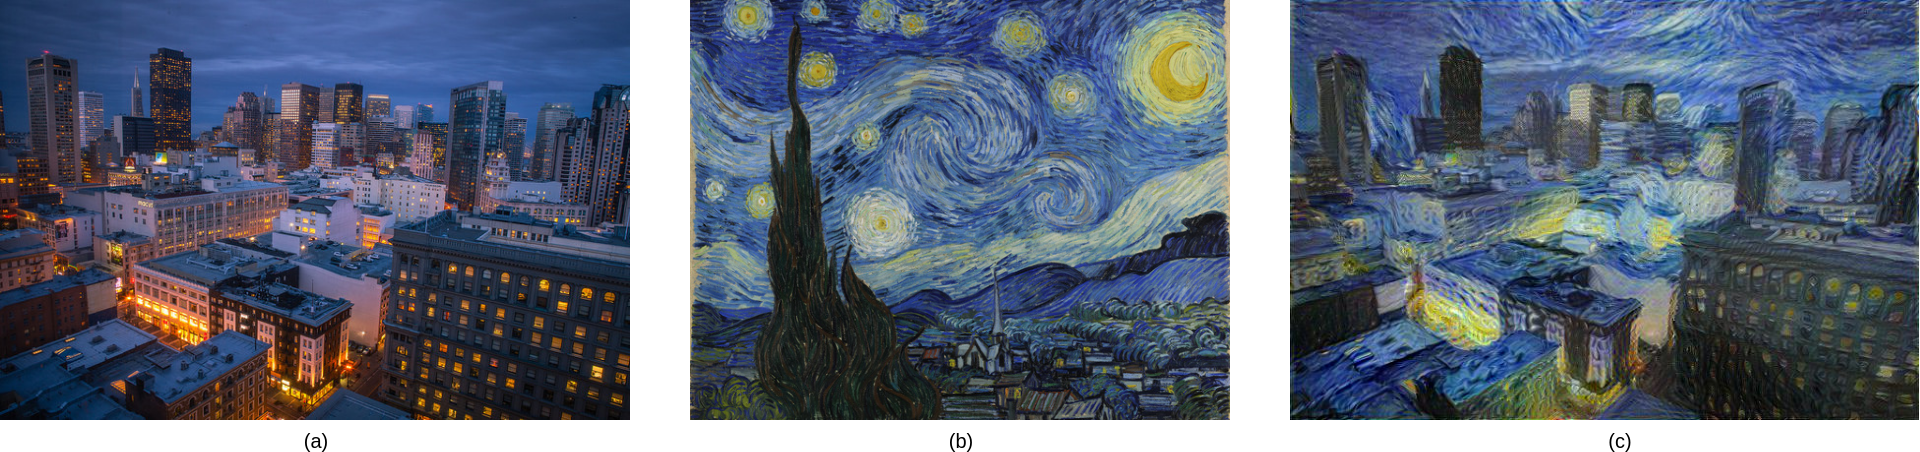
\includegraphics[width=\textwidth]{images/style-transfer-vision.png}
    \imgsrc{\url{https://github.com/fzliu/style-transfer}}
	\caption{\label{fig:style-transfer-vision}Sample of vision style transfer. Image (a) provides the content, image (b) provides the style and image (c) is the final generated image}
\end{figure}


\begin{table}[ht]
	\centering
	\begin{tabular}{ | p{.45\linewidth} | p{.45\linewidth} | }
		\hline
		\textbf{Input}                                              & \textbf{Output}                                      \\
		\hline \hline
		i will bite thee by the ear for that jest .                 & i ’ ll bite you by the ear for that joke .           \\
		\hline
		what further woe conspires against mine age ?               & what ’ s true despair conspires against my old age ? \\
		\hline
		how doth my lady ?                                          & how is my lady ?                                     \\
		\hline
		hast thou slain tybalt ?                                    & have you killed tybalt ?                             \\
		\hline
		an i might live to see thee married once , i have my wish . & if i could live to see you married, i ’ ve my wish . \\
		\hline
		benvolio , who began this bloody fray ?                     & benvolio , who started this bloody fight itself ?    \\
		\hline
		what is your will ?                                         & what do you want ?                                   \\
		\hline
		call her forth to me .                                      & bring her out to me .                                \\
		\hline
	\end{tabular}
	\imgsrc{\cite{xu2012paraphrasing}}
	\caption{Results of transferring authorship style from Shakespearean plays to modern english}
	\label{tab:paraphrasing-for-style-results}
\end{table}

This problem in the context of text was first introduced in by \cite{xu2012paraphrasing} as a statistical model that attempted to paraphrase bodies of text in a different style using a simple replacement strategy. An few examples from this paper are shown in Table \ref{tab:paraphrasing-for-style-results}. Since the overwhelming adoption of neural network based models in the NLP community, there have been several new bodies of work that break new ground in this area.


\section{Problem Statement}

The objective of this thesis is to perform an exploratory analysis of previous methods and test novel hypotheses that tackle the problem of the disentanglement of latent spaces of artificial neural networks and its applications to linguistic style transfer.

We operate under the following constraints and assumptions in our formulation of the problem:

\begin{itemize}
	\item The model is singular, with no conditional execution branch based on desired attribute. i.e. there is only one decoder and the number of decoders does not scale with the number of distinct transferrable attributes.
	\item The corpus of styles are non-parallel i.e. for instance, there are no pre-defined pairs of $(document_1, document_2)$ for style labels $\in (1, 2)$, as would be commonly seen in neural machine translation corpora.
	\item The corpora is annotated with the current attribute each document possesses e.g. each document has a corresponding `positive'/`negative' label if the task is to perform sentiment transfer.
	\item Optionally, a lexicon of words that are statistically very likely to be associated with each distinct class label would be useful, primarily to evaluate how well content has been preserved without penalizing change in vocabulary caused by the transferring of style.
\end{itemize}

The next chapter will delve deeper into the background required for an understanding of the models we implement and evaluate.


%======================================================================
\chapter{Background}
%======================================================================

\section{Natural Language Generation}

Natural Language Generation (NLG) is a sub-field of Natural Language Processing that attempts to generate sequences of words that resemble natural human languages. Traditionally, this was done either by using production rules of a predefined grammar, or by performing statistical analyses of existing human-written texts to predict sequences of words, based on their occurrence probabilities \citep{cambria2014jumping}. Markov-chain text generators are an example of the latter, popularized by their usage in parody text generation \citep{jelinek1985markov}.

This broad classification of problems has multiple applications including, but not limited to:
\begin{itemize}
	\item Neural machine translation (NMT), in which the generation objective is to produce a semantically similar sentence in a target language, given a sentence in a source language \citep{bahdanau2014neural,cho2014properties,luong2015effective,wu2016google}.
	\item Dialogue generation, in which the objective is to produce a natural and syntactically correct response to a provided utterance \citep{cavazza2005dialogue,li2016persona,li2016deep,li2017adversarial}.
	\item Text summarization, which eliminates superfluous and non-pertinent information in a body of text, to express the idea using fewer words \citep{barzilay1999using,gong2001generic,conroy2001text}.
	\item Data-to-text report generation, which utilizes structured data, sourced from a relational data format, to fill out a text template \citep{goldberg1994using,reiter2007architecture,gatt2009data}.
\end{itemize}


\section{Multi-Layer Perceptrons}

Multi-layer perceptrons (MLP) are widely used in the neural network literature as the simplest vanilla artificial neural network. An MLP typically comprises one or more hidden layers that learn intermediate representations before producing an output layer. A simple MLP classification architecture for MNIST digits \citep{lecun2010mnist,deng2012mnist} is depicted in Figure \ref{fig:mlp-network}. The network is represented as a directed graph containing nodes and edges, where each node represents a neuron and each edge represents a learned weight. Each weight here is a model parameter. In this example, the weight between two successive layers are densely interconnected. Given a layer of $m$ nodes and a subsequent layer of $n$ nodes that are densely connected, we require $m*n$ edges (or weights) to connect the nodes of these two layers. These $m*n$ edges form a matrix representing the model parameters that transform a vector represented in the first layer to a vector represented in the second layer.

\begin{figure}[ht]
	\centering
	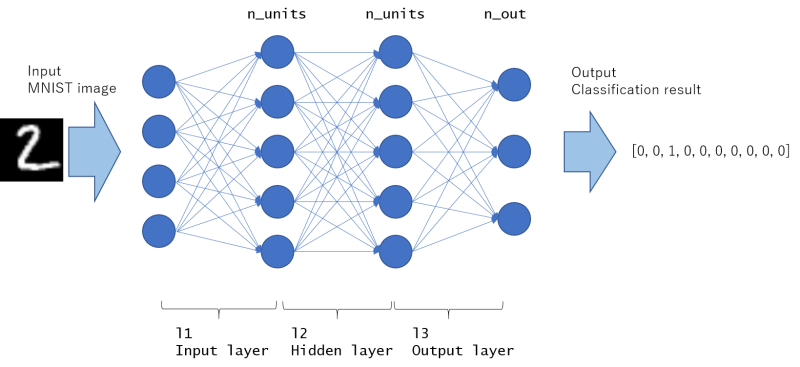
\includegraphics[width=\textwidth]{images/mlp-network}
	\imgsrc{\url{http://corochann.com/mnist-training-with-multi-layer-perceptron-1149.html}}
	\caption{\label{fig:mlp-network} Multi-Layer Perceptron}
\end{figure}

In terms of function approximation, a multilayer perceptron can be thought of as nested function calls on the input $x$. For example, assume that the intermediate layers approximate the functions $f_1$ and $f_2$, and the output layer approximates the function $f_3$ in the example presented in Figure \ref{fig:mlp-network}. We can then say that the relation of the output distribution $y$ with respect to the features in the input sample $x$ would be described as $y = f_3(f_2(f_1(x)))$. The back-propagation of the objective loss over the weights of the network is achieved by using the chain-rule to differentiate this nested function. The gradients thus obtained are then used to update the weights, thereby changing how the output layer is computed during the next iteration of computation through the directed graph \citep{lecun1989backpropagation}.

The activation functions applied at each layer could either be linear or non-linear. The most popularly used non-linear activation functions are sigmoid, tanh, ReLU etc., which are typically used in the intermediate layers of the network. In the case of multi-label prediction problems, the output layer is typically a softmax distribution over the possible output classes. The softmax activation is simply the binary logistic regression classifier that generalizes to multiple classes, since the output of the softmax function can be used to represent a categorical distribution (Equation \ref{eqn:softmax-function}).

\begin{equation} \label{eqn:softmax-function}
	P(y=j \mid \mathbf{x}) = \frac{e^{\mathbf{x}^\mathsf{T}\mathbf{w}_j}}{\sum_{k=1}^K e^{\mathbf{x}^\mathsf{T}\mathbf{w}_k}}
\end{equation}

An MLP classifier is trained by minimizing a cross-entropy loss between the predicted softmax distribution $y$ and the true distribution $y'$
\begin{equation}
	\mathcal{H}_{y'} (y) := - \sum_{i}^K y_{i}' \log (y_i)
\end{equation}
where $K$ is the total number of classes.


\subsection{Dropout}

Dropout is a regularization technique used during the training of neural networks. It was proposed by \cite{srivastava2014dropout} as a simple method to prevent a model from over-fitting the approximately learned function on the training data. The idea of dropout is to randomly ignore a set of neural network weights i.e. randomly set function parameters to 0 during each instance of the forward pass, as shown in Figure \ref{fig:dropout}.

\begin{figure}[ht]
	\centering
	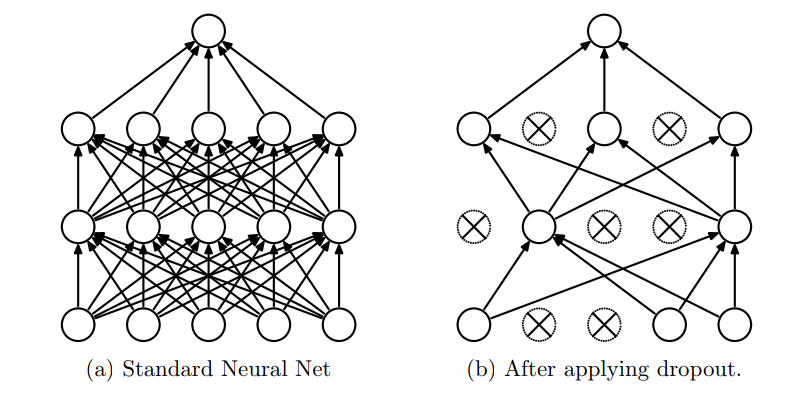
\includegraphics[width=\textwidth]{images/dropout}
	\imgsrc{\cite{srivastava2014dropout}}
	\caption{\label{fig:dropout} Dropout}
\end{figure}

Each neuron / unit is dropped out with a predefined probability, which can be viewed as a model hyperparameter. This allows for more generalized and robust functions being learned by minimizing the co-dependence of neurons on each other. Dropout has also been empirically shown to improve experiment results on several supervised learning tasks in vision, speech recognition, document classification and computational biology \citep{srivastava2014dropout}.


\section{Convolutional Neural Networks}

A convolutional neural network (CNN) \citep{lecun1995convolutional} is a specialized neural network that is optimized for feature extraction from local regions in data, for instance a specific object in an image, or a specific attribute in a body of text. Using densely connected multi-layer perceptrons for feature extraction from all the pixels of an image increases the number of parameters and slows down the training process. Instead, convolutional networks use shared weights over the source data that are called `filters'.

The `convolution' within a convolutional neural network is implemented using a filter. A filter is a learned function that transfers an arbitrary spatial representation of the image, say $3\text{px} * 3\text{px}$, into a single value and this is done for all the similar spatial zones in the image. 2-dimensional convolutions are used to process features in images and video because of their inherent spatial nature. A 1-dimensional equivalent could be used to extract features from contiguous regions of text, usually 3 to 5 words \citep{kim2014convolutional}. These features are then sub-sampled to reduce the dimensionality for subsequent layers. This is typically achieved by max-pooling or average-pooling, which simply requires aggregating all the spatially proximal region activations produced by the convolutional layer.

The strategy of stacking convolutional and pooling layers allows the network to learn parameters that are translation invariant. In simpler words, an object can be identified regardless of its location in an image, and an attribute can be identified regardless of its position in a body of text.

An example CNN architecture is presented in Figure \ref{fig:cnn}.

\begin{figure}[ht]
	\centering
	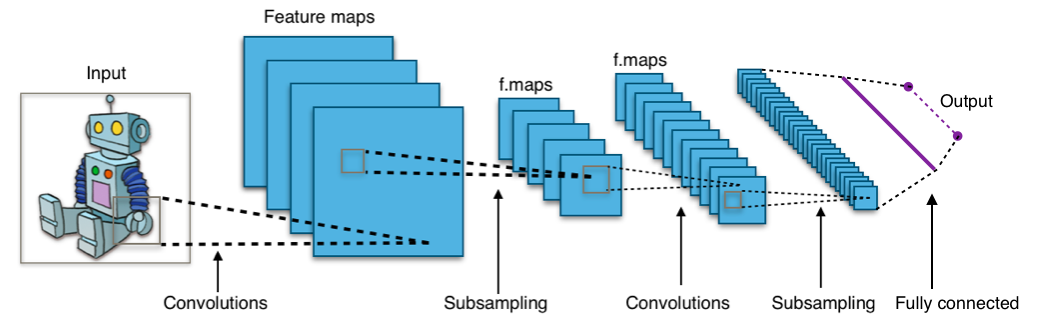
\includegraphics[width=\textwidth]{images/cnn}
	\imgsrc{\url{https://commons.wikimedia.org/wiki/File\%3ATypical_cnn.png}}
	\caption{\label{fig:cnn} Convolutional Neural Network}
\end{figure}

Since their inception, CNNs have been proven to achieve state-of-the-art results in multiple task settings within vision and language, especially with the use of deep convolutional architectures \citep{lawrence1997face,krizhevsky2012imagenet,karpathy2014large,kalchbrenner2014convolutional,kim2014convolutional,hu2014convolutional}.


\section{Recurrent Neural Networks}

Recurrent neural networks (RNNs) are a sub-class of artificial neural networks that are commonly used for sequence processing. Its units forms a directed graph that operates on a sequence of inputs in a temporally-distributed manner. This makes them a useful tool for extracting features from arbitrary length sequences of input like audio or text. The optimization problem an RNN tries to solve is to predict the next element in a sequence given the historical context, as shown in Equation \ref{eqn:rnn-next}.
\begin{equation} \label{eqn:rnn-next}
	P(w_1, \cdots, w_T) = \prod_{i=1}^T P(w_i | w_1, \cdots, w_{i-1})
\end{equation}

The language model is built in such a way that the features extracted from the sequence at time-step $t$ depend on the features observed during the time-steps $0 \cdots t-1$. A graphical depiction of a temporally-unrolled RNN is shown in Figure \ref{fig:recurrent-neural-network-unfold}.

\begin{figure}[ht]
	\centering
	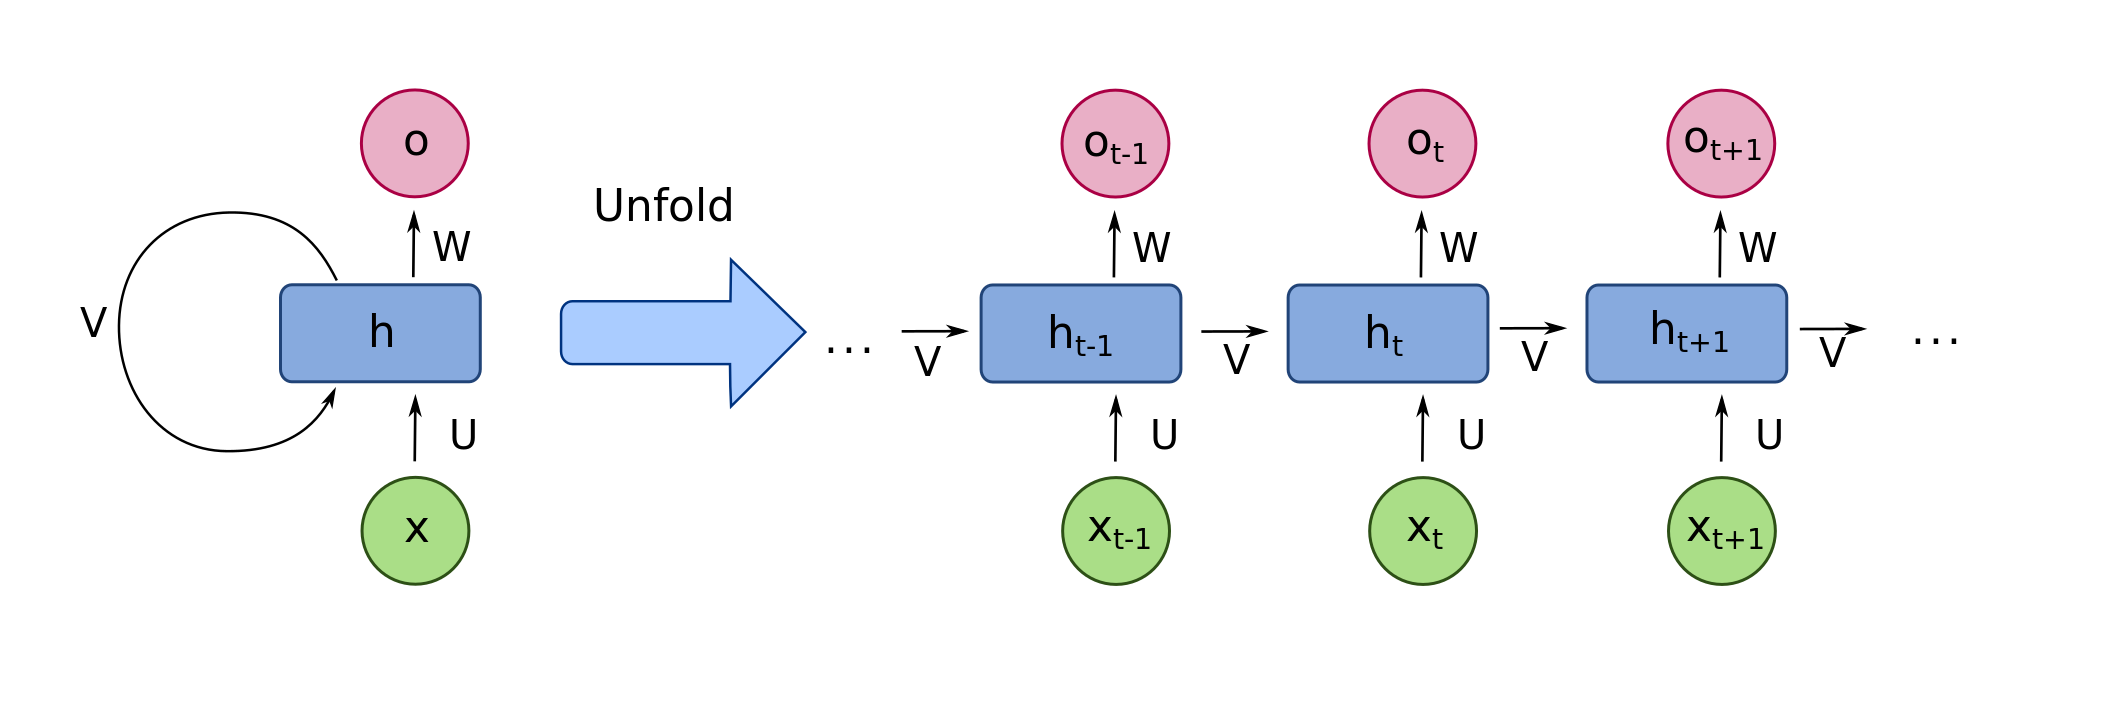
\includegraphics[width=\textwidth]{images/recurrent-neural-network-unfold}
	\imgsrc{\url{https://commons.wikimedia.org/wiki/File:Recurrent_neural_network_unfold.svg}}
	\caption{\label{fig:recurrent-neural-network-unfold} Recurrent Neural Network}
\end{figure}

The most recent and useful variants of recurrent units provide the ability to retain `memory' of the context in which the current features are to be extracted. In the domain of language processing, this typically implies that the recurrent unit has a stored memory of the previously observed words in a sequence, and this property grants it the ability to learn context as part of the feature space. The prominent variants of recurrent units used in neural networks to extract features from sequences using a memory mechanism, are Long Short-Term Memory (LSTM) units \citep{gers2001lstm} and Gated Recurrent Units (GRU) \citep{chung2014empirical}.

Recurrent networks in the domain of natural language processing are used frequently for both natural language understanding (NLU) tasks, as well natural language generation (NLG) tasks \citep{bengio2003neural,morin2005hierarchical,mikolov2010recurrent}. Similar to the manner in which recurrent networks can extract features from arbitrarily long sequences of vectorized text, they can also be used to produce text sequences from a unit vector representation of text, as represented in Figure \ref{fig:rnn-nmt}.

This is achieved by conditioning the generation of the first word of text either on some latent variable produced by a model, or by sampling from a generative distribution, and conditioning the generation of each subsequently predicted word on the word that was predicted in the previous time-step, until the model predicts an end-of-sentence (EOS) token.

\begin{figure}[ht]
	\centering
	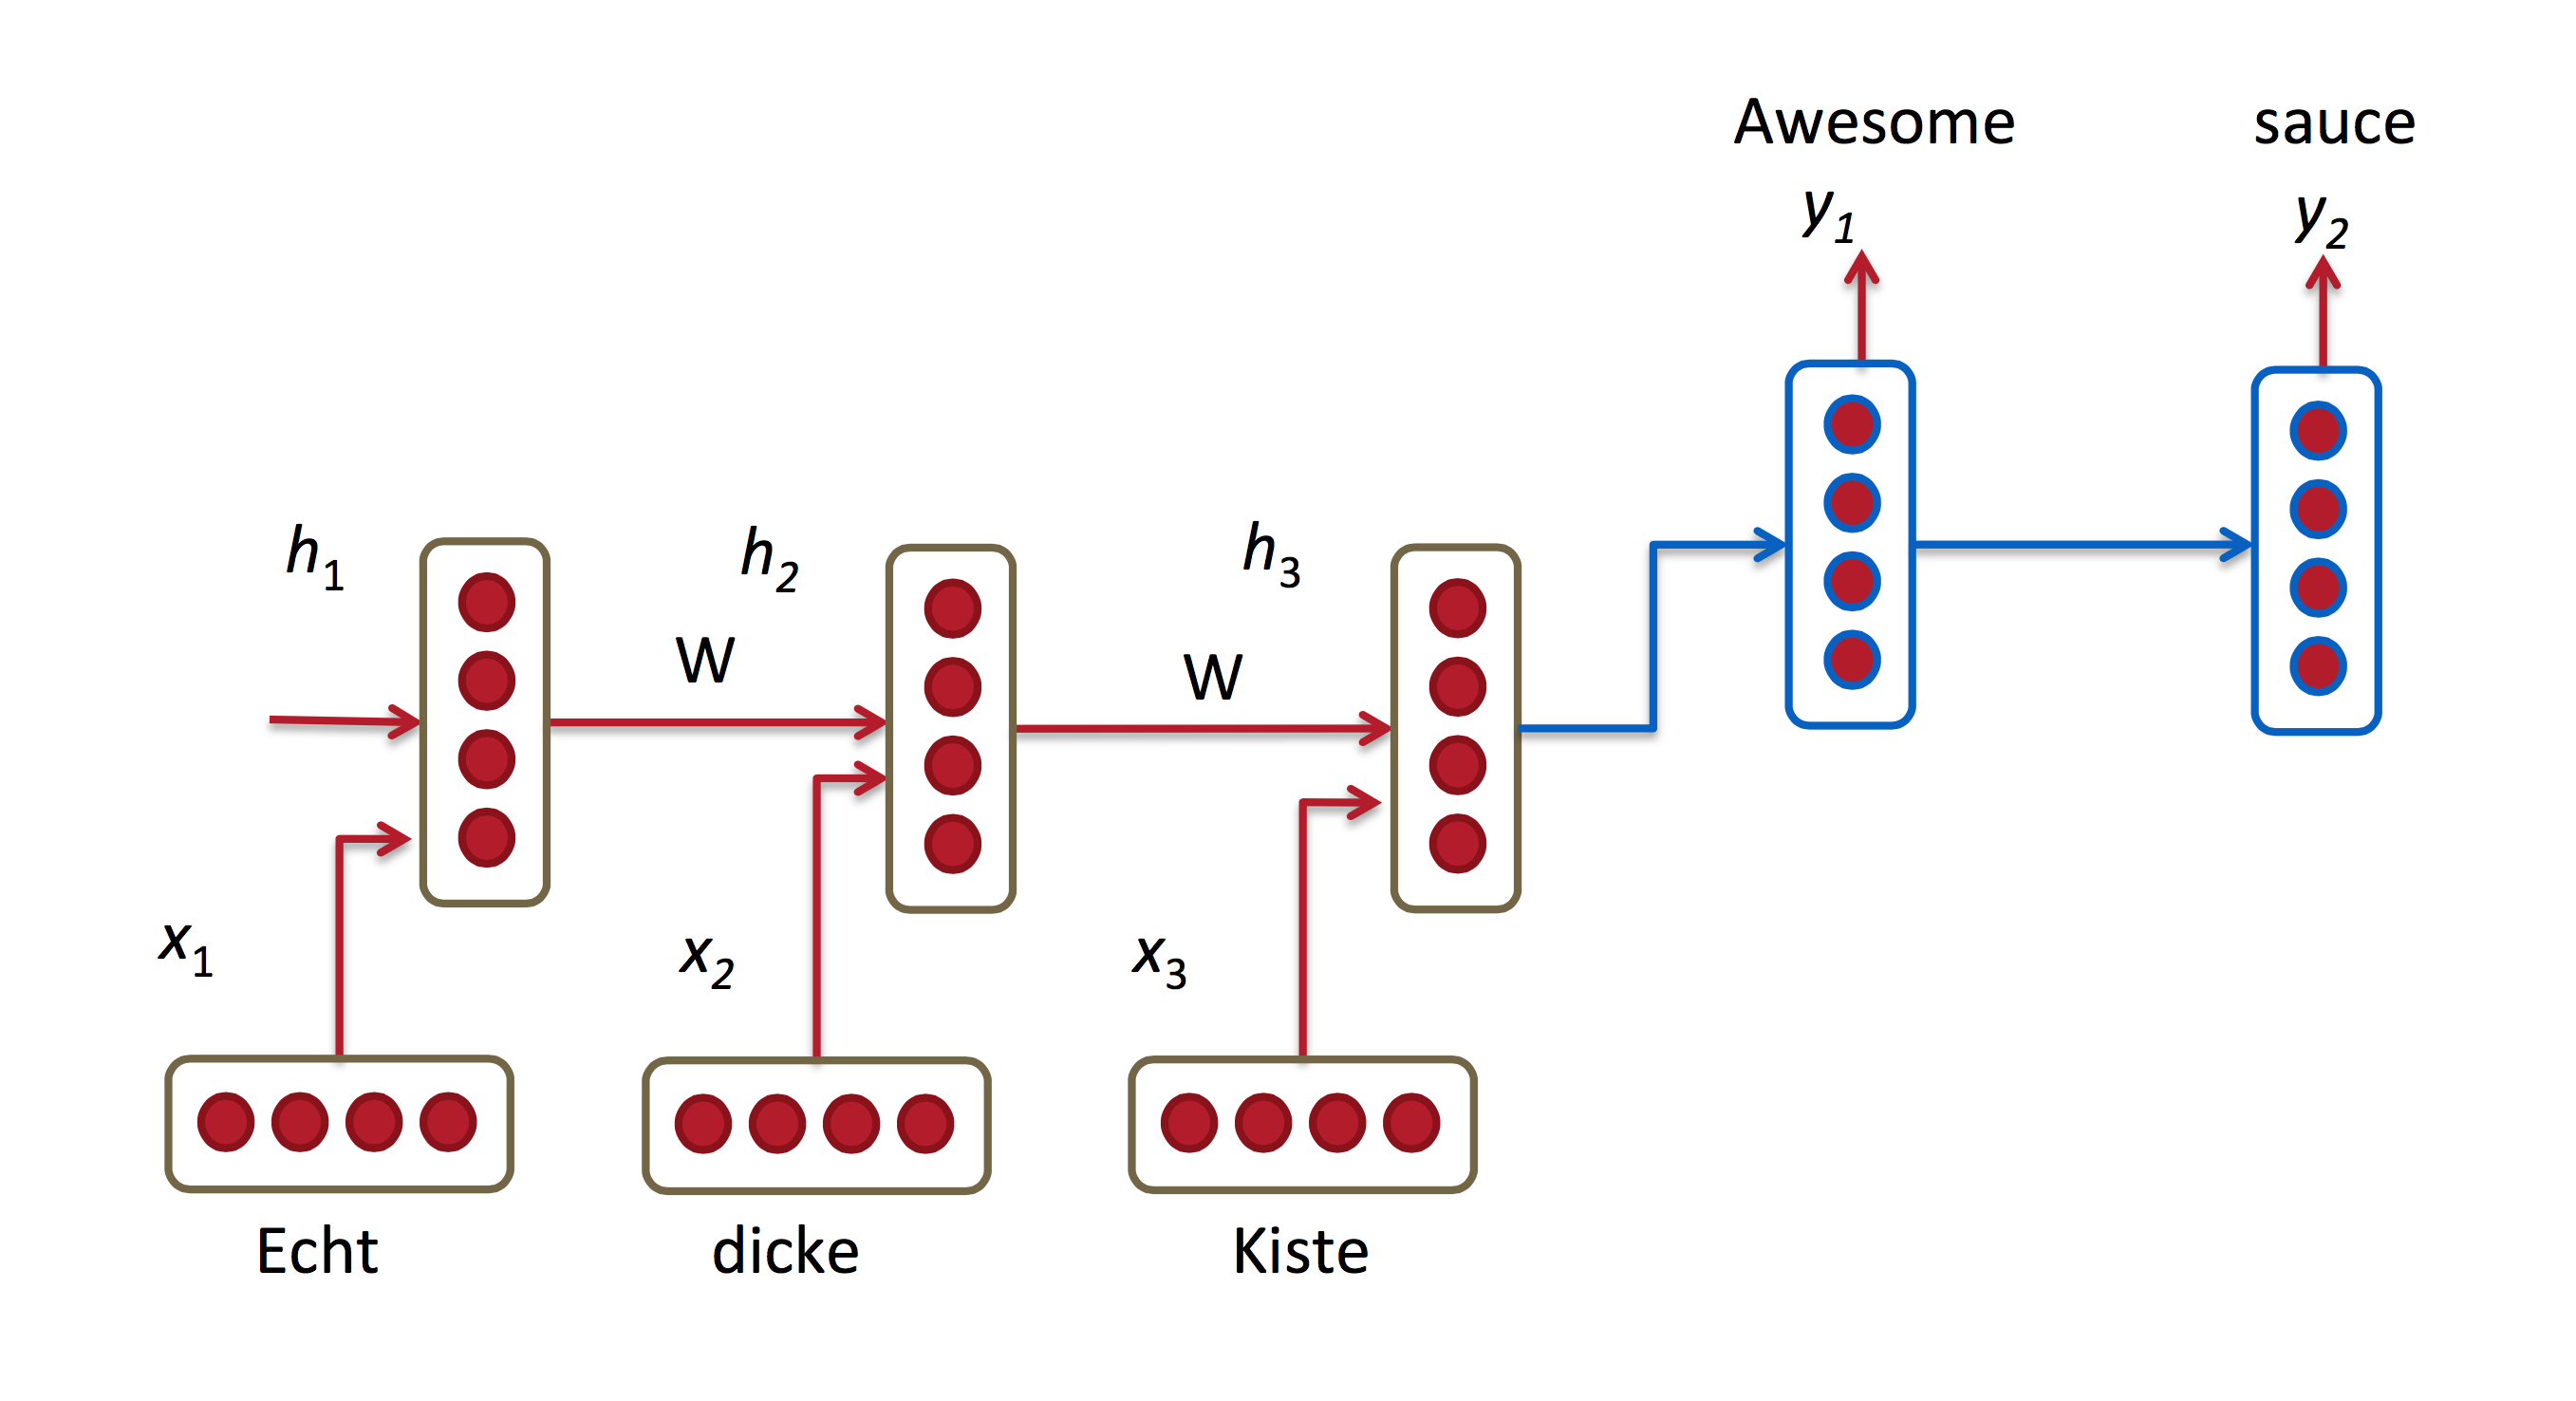
\includegraphics[width=\textwidth]{images/rnn-nmt}
	\imgsrc{\url{http://www.wildml.com/2015/09/recurrent-neural-networks-tutorial-part-1-introduction-to-rnns}}
	\caption{\label{fig:rnn-nmt} Recurrent Encoder-Decoder Model}
\end{figure}


\subsection{Long Short-Term Memory}

As described in the previous section, recurrent neural networks (RNN) learn representations of the data over temporal sequences, like text or audio features. However, in practice, RNNs don't seem to be able to assign priorities to which of the past data they choose to ascribe a higher importance to. This is detrimental to their usage in tasks that require processing of long sequences of data like in text, audio or video processing. This lack of ability to learn long-term dependencies in the input features is shown in previous work by \cite{bengio1994learning}.

Long Short-Term Memory (LSTM) units, as described first by \cite{hochreiter1997long}, seek to address this issue by explicitly modelling how much to retain and forget at each time-step during the RNN's training procedure.

\begin{figure}[ht]
	\centering
	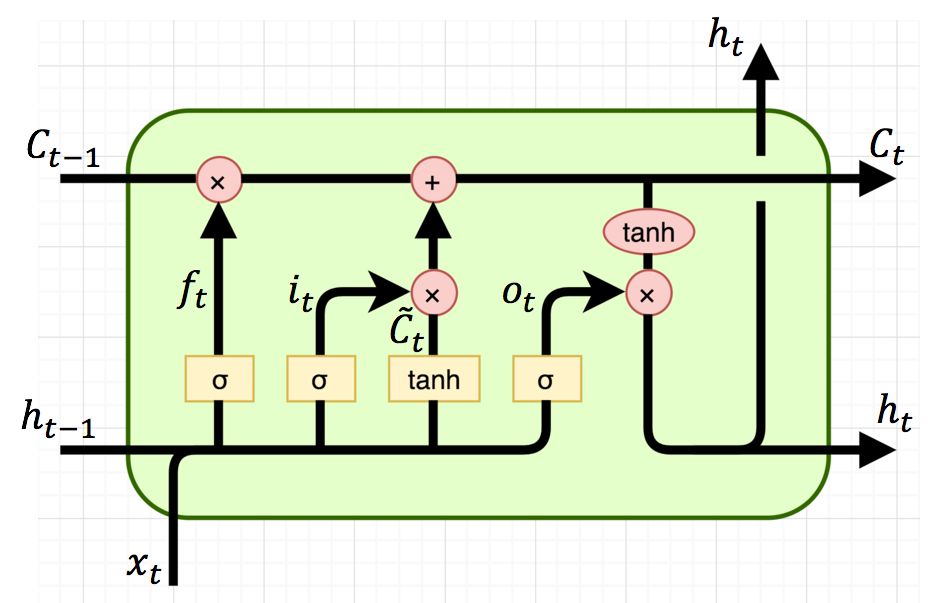
\includegraphics[width=\textwidth]{images/lstm}
	\imgsrc{\url{https://isaacchanghau.github.io/post/lstm-gru-formula}}
	\caption{\label{fig:lstm} Long Short-Term Memory Unit}
\end{figure}

The structure of an LSTM is depicted in Figure \ref{fig:lstm}. An LSTM is comprised of three distinct gating layers internally - namely the forget gate, input gate and output gate - that determine its outputs: the new cell state and hidden state. As can be seen in Figure \ref{fig:lstm}, the cell state $C_t$ passes through the LSTM mostly unperturbed, which is intended to address the problem of vanishing gradients \citep{hochreiter1999vanishing}.

The forget gate uses a sigmoid activation to squash the values of the output of the previous time-step between 0 and 1, which can be understood as being semantically equivalent to deciding how much of the previous cell state to forget.
\begin{equation*}
	f_t = \sigma(W_f*[h_{t-1}, x_t] + b_f)
\end{equation*}

The input gate also uses a sigmoid activation on the previous hidden state, which is multiplied by the candidate cell state $\hat{C_t}$. The value thus obtained is then multiplied by the forget-gated previous cell state to form the next cell state.
\begin{align*}
	i_t =
	 & \sigma(W_i*[h_{t-1}, x_t] + b_i) \\
	\hat{C_t} =
	 & \tanh(W_c*[h_{t-1}, x_t] + b_c)  \\
	C_t =
	 & f_t * C_{t-1} + i_t * \hat{C_t}
\end{align*}

Now that we have obtained the cell state, we propagate that through to the next time-step. To obtain the hidden state, we use an output gate, again with a sigmoid activation, to gate the cell-state and create the hidden-state for the next time-step.
\begin{align*}
	o_t =
	 & \sigma(W_o*[h_{t-1}, x_t] + b_o) \\
	h_t =
	 & \tanh(C_t)
\end{align*}

The efficacy of LSTM-backed RNNs is evident from the prevalence of their usage in language modelling literature \citep{sundermeyer2012lstm,gers2001lstm,graves2005framewise} \footnote{\url{https://karpathy.github.io/2015/05/21/rnn-effectiveness}}.

\subsection{Gated Recurrent Units}

Gated Recurrent Units (GRU) \citep{cho2014learning} are similar to LSTMs in that they possess gating mechanisms to assist with long-term dependency learning. They differ from LSTMs in a few aspects, like the merging of the input and forget gates into a single update gate. They also merge cell state and hidden state, emitting only a single output vector after the computations within the cell. Figure \ref{fig:gru} depicts the internal GRU states and gates.

\begin{figure}[ht]
	\centering
	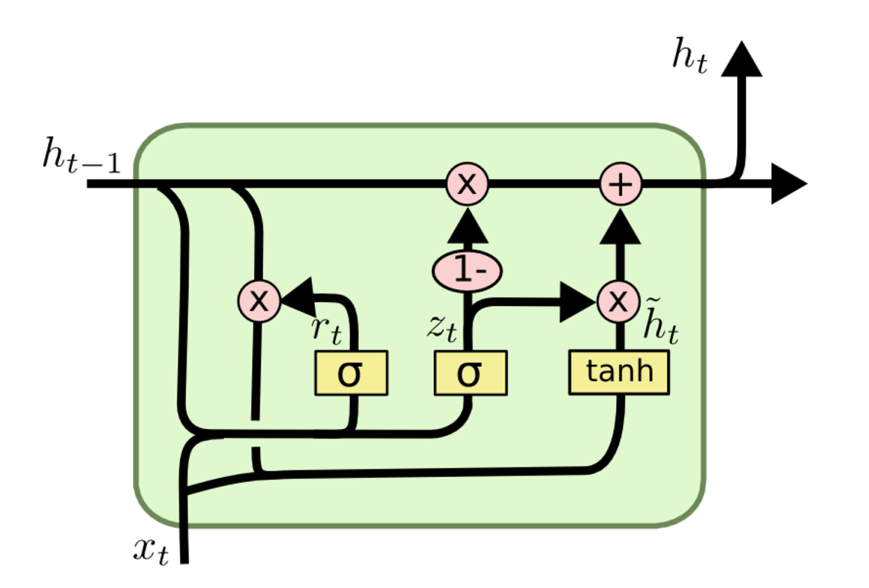
\includegraphics[width=\textwidth]{images/gru}
	\imgsrc{\url{https://isaacchanghau.github.io/post/lstm-gru-formula}}
	\caption{\label{fig:gru} Gated Recurrent Unit}
\end{figure}

GRUs are a lot simpler to work with in practice due to their having only a single output. They have been used interchangeably with LSTMs as memory units for recurrent neural networks \citep{chung2015gated,fu2017style}.


\section{Autoencoders}

Autoencoders are models that are parameterized to convert arbitrary data into a latent representation (encoder), and recover the original data back from the latent representation (decoder). In this setup, the dimensionality of the latent representation is usually much smaller than that of the actual data. A simple autoencoder architecture is depicted in Figure \ref{fig:autoencoder-structure}.

\begin{figure}[ht]
	\centering
	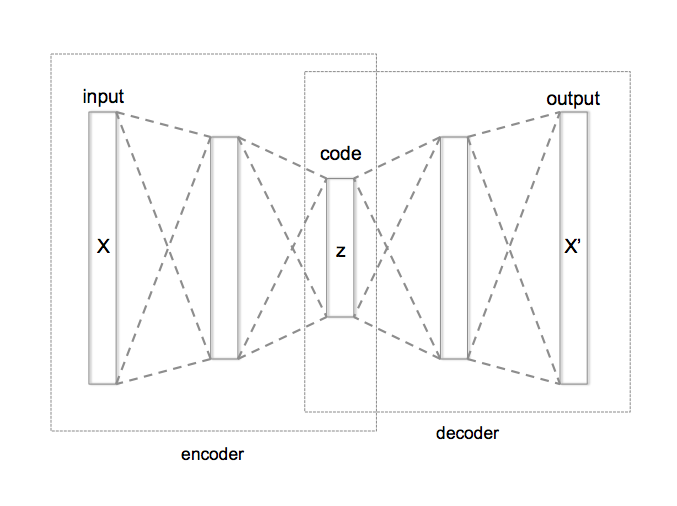
\includegraphics[width=\textwidth]{images/autoencoder-structure}
	\imgsrc{\url{http://mlexplained.com/2017/12/28/an-intuitive-explanation-of-variational-autoencoders-vaes-part-1}}
	\caption{\label{fig:autoencoder-structure} Model Architecture: Autoencoder}
\end{figure}

By training a model to reconstruct data that is funnelled through a lower dimensional representation, two objectives can be achieved simultaneously:
\begin{itemize}
	\item The encoder weights of the model could be used to extract the most salient features of the data in a compressed representation, which is a better input feature format for downstream processing or learning algorithms. \citep{hinton2006reducing}
	\item The decoder weights of the model could be used as a generator. Given that we can sample from the distribution of the existing latent representations learned, or from a predefined prior (in a variational autoencoder), we can generate plausible novel data.
\end{itemize}

In the context of natural language, the encoder can be utilized as a sentence-encoding feature-extractor and the decoder can be utilized as a generative model. Autoencoders are also able to de-noise data given pairs of noisy and regular data, by learning a de-noising function, which can then be used for actual noisy data. These properties make autoencoders a good framework to utilize to implement sequence-to-sequence models, wherein both the encoder and decoder weights of the model are parameterized by neural networks that process and generate sequences of data, respectively.

\subsection{Variational Autoencoders}

Variational autoencoders (VAEs) \citep{kingma2013auto} are a probabilistic variant of autoencoders. The general structure of a VAE is the same as that of a deterministic autoencoder, with an encoder that learns a compressed latent space and a decoder that learns a function to map the latent space into the original data. In contrast with the deterministic autoencoder, a variational autoencoder parameterizes representations of the latent mean and variance as separate spaces. The method of variational inference requires placing conjugate priors on the mean and variance of the hitherto unknown latent representation. The encoder is then trained to learn the approximate posterior distribution, and the decoder is trained to generate novel data using samples taken from the prior distribution. The family of distributions used for this purpose are Gaussian. A simple VAE architecture is depicted in Figure \ref{fig:vae-structure}.

\begin{figure}[ht]
	\centering
	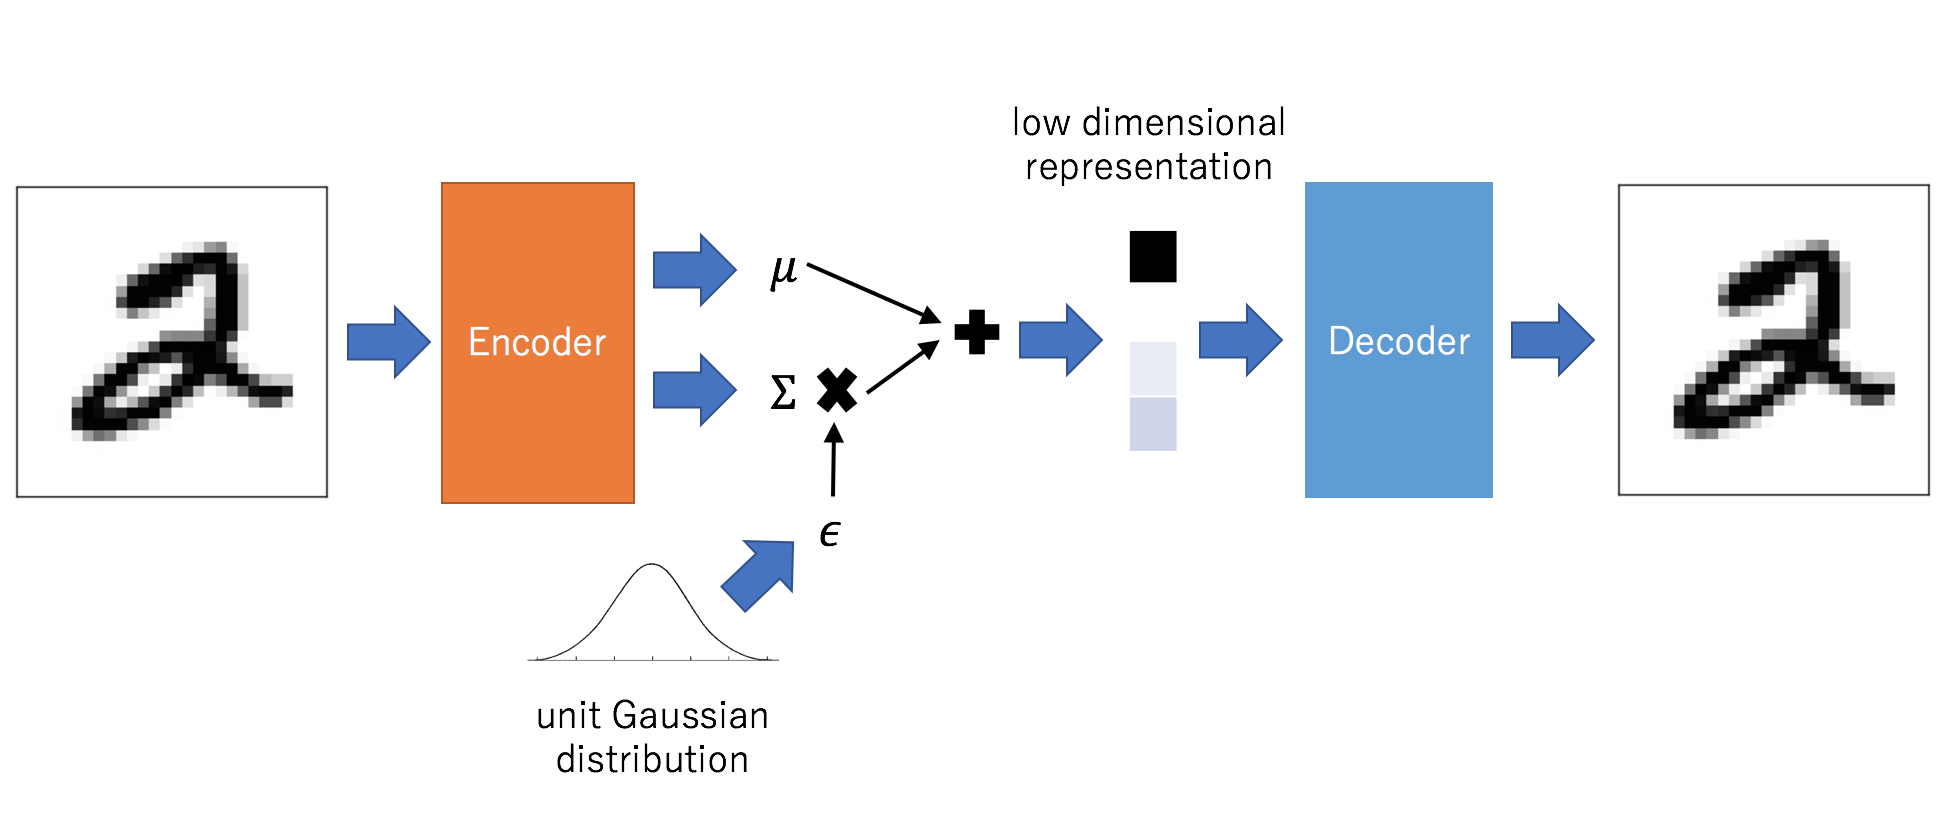
\includegraphics[width=\textwidth]{images/vae-structure}
	\imgsrc{\url{http://mlexplained.com/2017/12/28/an-intuitive-explanation-of-variational-autoencoders-vaes-part-1}}
	\caption{\label{fig:vae-structure} Model Architecture: Variational Autoencoder}
\end{figure}

In addition to the reconstruction loss that a deterministic autoencoder uses, a metric of distance is used to evaluate how closely the learned representations of mean and variance resemble a Gaussian distribution with mean 0 and unit variance. The Kullback-Leibler (KL) divergence \citep{kullback1951information} is used to penalize learned representations that do not resemble the prior. However, we cannot compute the KL divergence directly. Instead we compute an alternative objective that is equivalent to the KL divergence up until an added constant. This is called the evidence lower-bound (ELBO). The ELBO objective maximized in a variational autoencoder model is given in Equation \ref{eqn:elbo}:
\begin{equation} \label{eqn:elbo}
	ELBO(q) = \mathbb{E}_{q(z)} [(\log(p(x|z))] - \mathbb{KL}(q(z)||p(z))
\end{equation}

Simultaneously, for the decoding step, we sample from the prior, utilizing the re-parameterization trick to ensure that the model remains differentiable. As a result, the decoder is trained as a generative network that can randomly sample from the prior and generates plausible data that is similar to the input distribution. The decoder being able to act as a generative model independently is what sets a VAE apart from a deterministic autoencoder.


\section{Word Embeddings}

Prior to the usage of matrix factorization and neural models to learn continuous word representations, the numerical representations used for words and documents were one-hot representations, word-ngrams \citep{brown1992class} or tf-idf weighted statistics. Word-ngrams are useful for expressing probability distributions of word occurrences in a corpus. Higher order ngrams (bigrams, trigrams, four-grams etc.) also take into account the context of nearby words, and can be used to construct language models.

However, these methods use discrete word or character occurrence counts to represent words and documents, and these representations scale with the size of the input corpus vocabulary for word-based models. This makes discrete word representation based language models computationally inefficient for large corpora with diverse vocabularies. Character-based models, on the other hand, are liable to produce invalid words and don't work as well with recurrent memory units as words do \citep{bojanowski2015alternative}. These methods are also ineffective at modelling semantic inter-word relationships.

Word2Vec, which aims to alleviate these problems, is a vector space model that embeds words into a continuous space. Also, semantically similar words in Word2Vec are embedded in nearby spaces \citep{mikolov2013distributed,mikolov2013linguistic,le2014distributed}. Word2Vec can model the corpus vocabulary in two different ways, namely CBOW and Skip-gram. The CBOW model predicts a target word from context words, whereas the Skip-gram model does the opposite and predicts target words from a single context word. Both model types are shown in Figure \ref{fig:efficient-models}

\begin{figure}[ht]
	\centering
	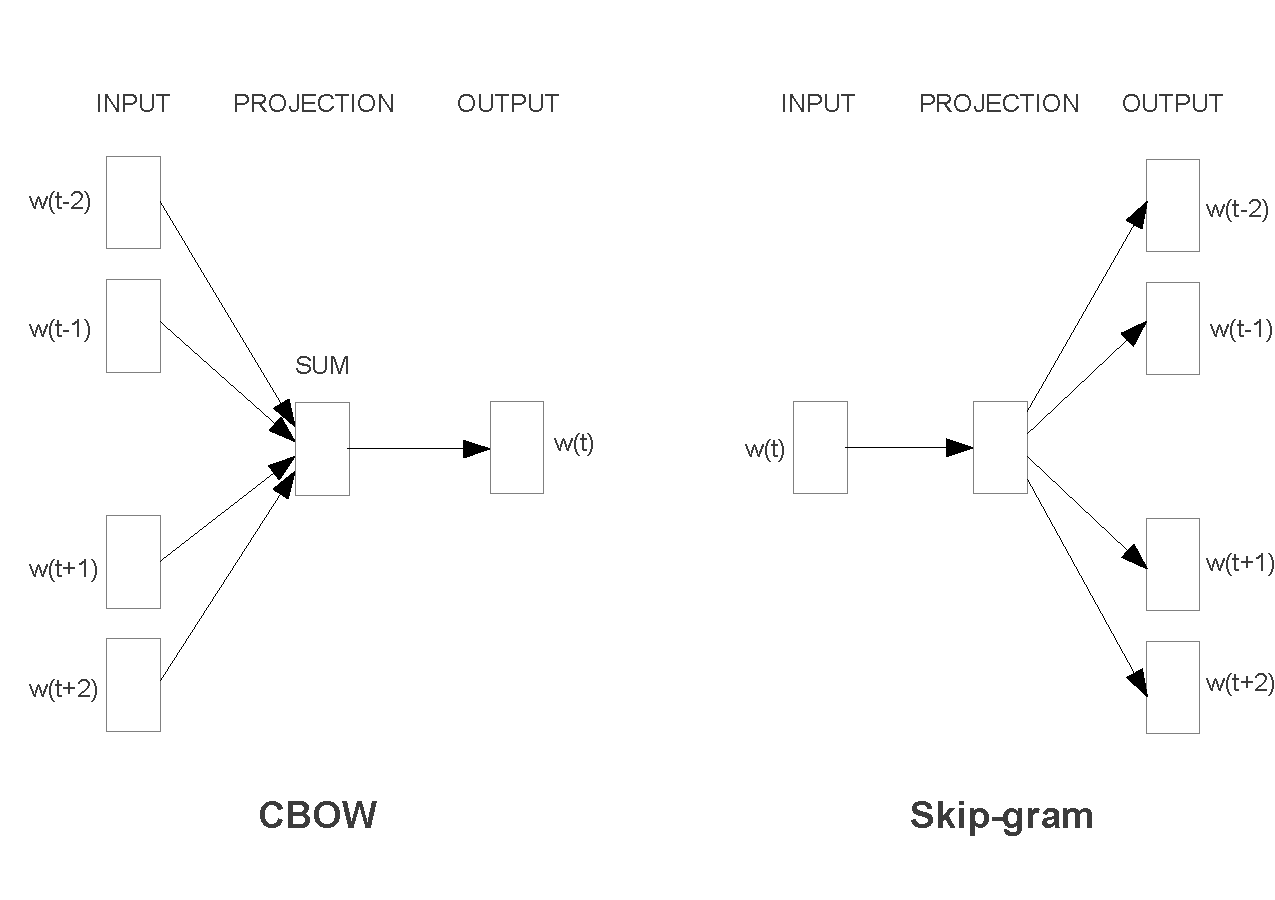
\includegraphics[width=\textwidth]{images/efficient-models}
	\imgsrc{\cite{mikolov2013efficient}}
	\caption{\label{fig:efficient-models} Word2Vec Model}
\end{figure}

The Word2Vec model is a simple shallow neural network, with single input, hidden and output layers. The hidden layer is of arbitrary size, called the embedding size. The embedding size is usually much lower that the vocabulary size, which is reminiscent of an autoencoder that learns a compressed salient representation of the words. The one-hot encoded input is transformed into its context or target word, depending on whether the algorithm chosen is CBOW or Skip-gram. This transformation is parameterized by the shallow neural network. After the model converges, the network weights connecting the input and the hidden layer can be used as parameters to obtain dense, continuous representations of words.

A surprising outcome of this embedding model is that translations within the learned vector space seem to emulate semantic (gender, tense) as well as factual relationships (country-capital), as shown in Figure \ref{fig:word2vec-linear-relationships}.

\begin{figure}[ht]
	\centering
	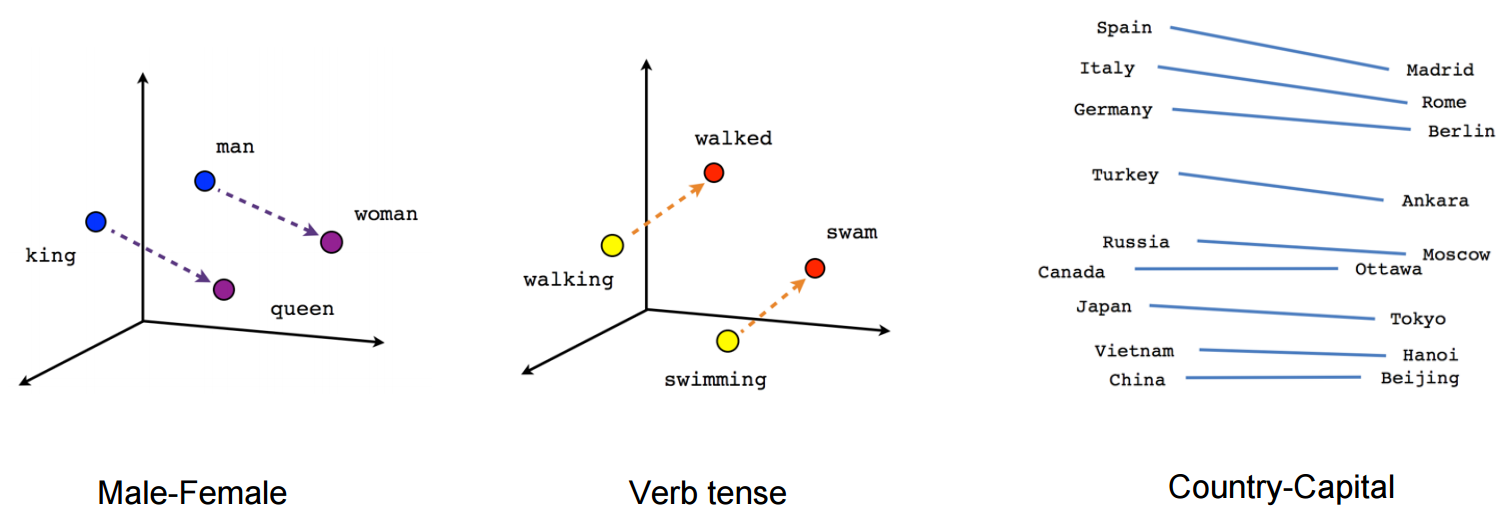
\includegraphics[width=\textwidth]{images/word2vec-linear-relationships}
	\imgsrc{\url{https://www.tensorflow.org/tutorials/word2vec}}
	\caption{\label{fig:word2vec-linear-relationships} Word2Vec Relationships}
\end{figure}

Word embedding neural models are also shown to be implicitly factorizing a word-context matrix by subsequent work in this area \citep{levy2014neural}.


\section{Sequence-to-Sequence Modelling}

Also abbreviated in the literature as Seq2Seq, this is a class of models that learns functions to transform one sequence into another. First introduced by \cite{sutskever2014sequence}, Seq2Seq is a flexible framework for modelling transformations made to arbitrary length sequences, typically using a neural encoder-decoder framework. In the field of natural language processing, the main tasks that benefit from such an encoder-decoder framework are those for which there exists two distinct distributions of text, and the model is trained to learn the mapping from one to the other.

\cite{sutskever2014sequence} define a sequence-to-sequence model that learns a function (Equation \ref{eqn:seq2seq}) to map a sequence of inputs $x_1, \cdots , x_T$ to a sequence of outputs $y_1, \cdots , y_{T'}$, where the initial state $h$ is set to the hidden LSTM representation of $x_1, \cdots , x_T$.

\begin{equation} \label{eqn:seq2seq}
	p(y_1, \cdots , y_{T'} | x_1, \cdots , x_T) =	\prod_{t=1}^T p(y_t | h, y_1, \cdots , y_{t-1})
\end{equation}

This makes the Seq2Seq model an ideal framework using which one can implement solutions to several natural language generation tasks like neural machine translation, dialogue generation, text summarization, etc.

\section{Generative Adversarial Networks}

\cite{goodfellow2014generative} presented a novel generative model that utilizes the idea of a game-theoretic competition between a generative model which is a decoder, and a discriminative model which is a classifier. The general idea is to train the discriminative model, also known as the adversary, to be able to discriminate between the synthetic distribution that the generator model produces, and a true distribution that the generator trying to mimic. Figure \ref{fig:gans} depicts a sample GAN model architecture.

\begin{figure}[ht]
	\centering
	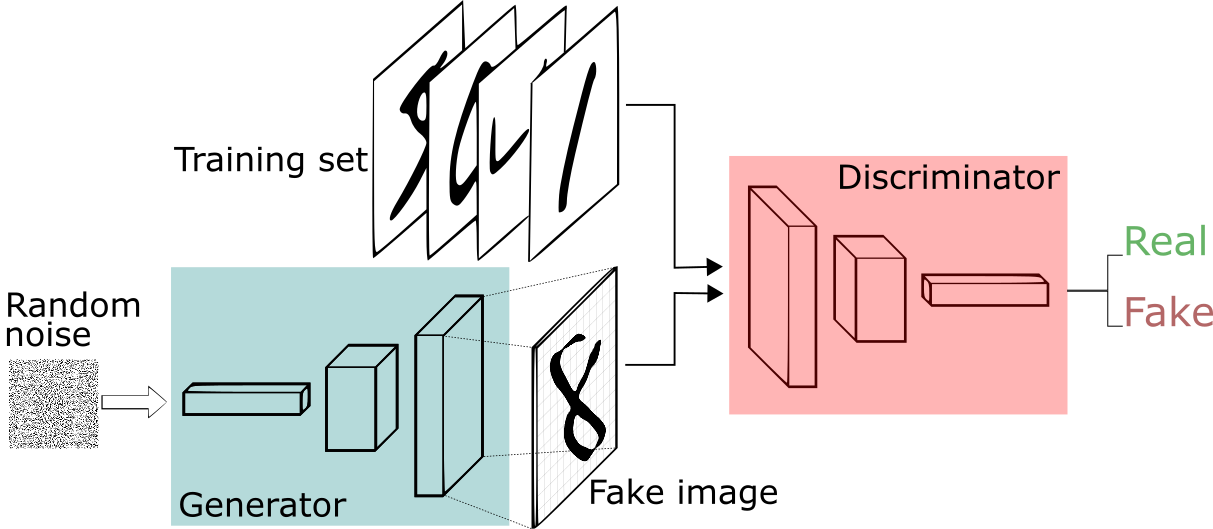
\includegraphics[width=\textwidth]{images/gans}
	\imgsrc{\url{https://deeplearning4j.org/generative-adversarial-network}}
	\caption{\label{fig:gans} Model Architecture: Generative Adversarial Networks}
\end{figure}

In the original formulation of adversarial training, which involves using a binary classifier, the generator learns weights to map a randomly initialized latent variable $z$ to a data distribution $x$ that it is unaware of. The discriminator is trained using the true distribution and samples generated by the generative model, with the objective to discriminate the true samples from the generated samples. The generator on the other hand, attempts to maximize the discriminator's classification error without directly modifying the discriminator's parameters, thereby producing plausible samples that mimic the true distribution. In this manner, both the generator and discriminator are simultaneously trained to both produce better synthetic samples, as well as differentiate between real and synthetic samples respectively. This min-max game is represented by Equation \ref{eqn:gan-minimaxgame}, where $D$ is the discriminator, $G$ is the generator and $V$ is the value-function or loss-function of the generative model.

\begin{equation}
	\label{eqn:gan-minimaxgame}
	\min_G \max_D V(D, G) = \mathbb{E}_{\bm{x} \sim p_{\text{data}}(\bm{x})}[\log D(\bm{x})] + \mathbb{E}_{\bm{z} \sim p_{\bm{z}}(\bm{z})}[\log (1 - D(G(\bm{z})))].
\end{equation}

This property the generator model's parameters possess - of translating random noise into plausible data samples - is used in areas of research within computer vision and natural language processing to produce novel data samples. Also, adversarial learning as a principle is an effective tool to ensure that a feature space is devoid of any arbitrarily chosen set of known attributes. We use this property of adversarial learning in our model to assist with the disentanglement of stylistic attributes.


\section{Visual Style Transfer}

The idea of neural style transfer was originally proposed by \cite{gatys2016image}. In the task described in the paper, the authors use two distinct images as input. The first image contributes the content, and the second contributes the style. The objective is to generate a final image that contains all of the physical objects visible in the first image, but depicted in the style (hue, brush strokes, texture, etc.) visible in the second.

\begin{figure}[ht]
	\centering
	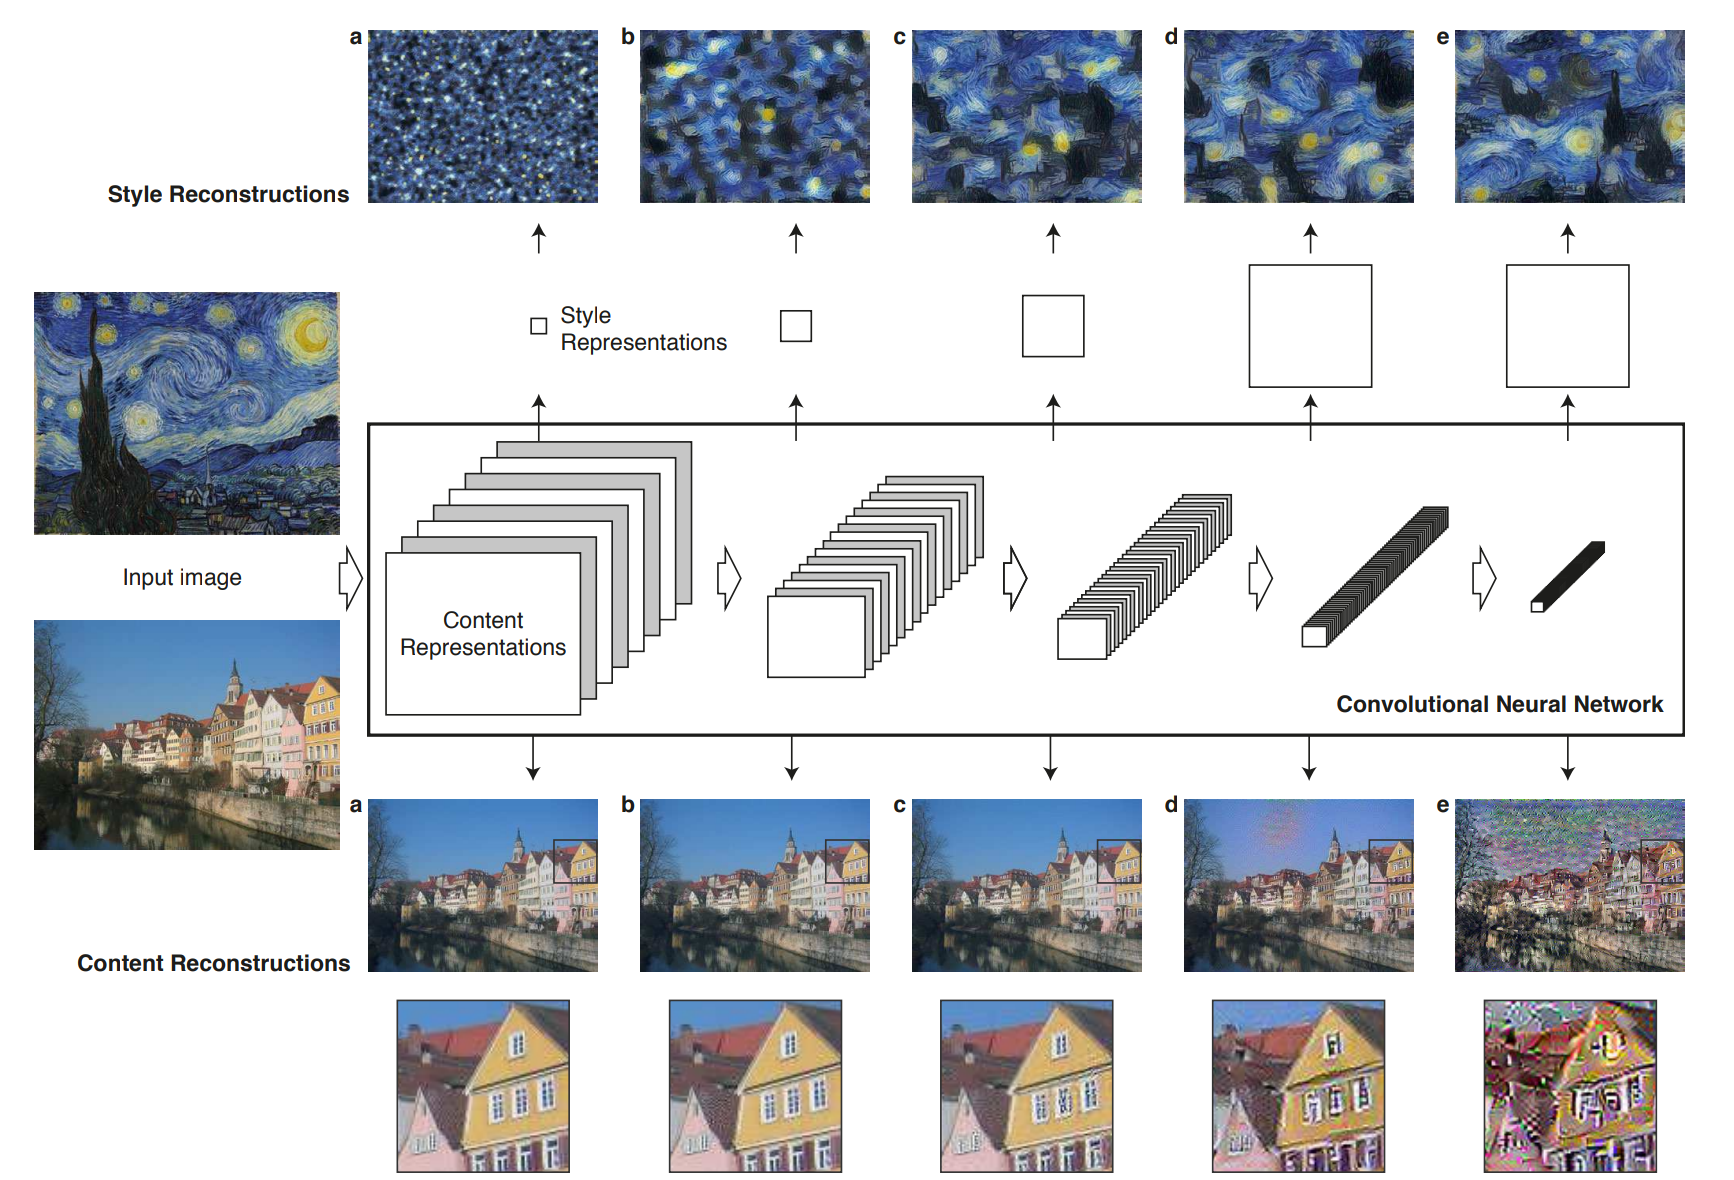
\includegraphics[width=\textwidth]{images/image-style-transfer}
	\imgsrc{\cite{gatys2016image}}
	\caption{\label{fig:image-style-transfer} Artistic Style Transfer in Images}
\end{figure}

The features, as with most of the state-of-the-art image processing techniques, are extracted from the images using Convolutional Neural Networks (CNNs) \citep{lecun1998gradient}, the deep neural network variants of which have been widely successful at image recognition tasks such as object recognition in the ImageNet dataset \citep{krizhevsky2012imagenet}.

As depicted in Figure \ref{fig:image-style-transfer}, subsequent layers of the CNN learn incrementally higher level features in both the style image and the content image. These learned features for the style and content images are stored for future use. To generate the final image, the authors begin with a random white noise image. This image is passed through both networks, the parameters of which extract both its style features and its content features.

This model uses two training objectives:
\begin{itemize}
	\item Minimize the the element-wise mean squared difference between the style features computed for the style image and the white-noise image.
	\item Minimize the the mean squared difference between the content features of the content image and the white noise image.
\end{itemize}

The overall training loss is a linear combination of the above objectives, and is used to iteratively modify the white-noise image until it has the style features of the style image and the content features of the content image.


In this chapter, we discussed the background needed to understand the methods used in our research and other related work. The next chapter builds on the fundamentals established here, and discusses previous attempts at neural disentanglement in the context of linguistic style transfer, as well as methods that do not use disentanglement as the basis of their style transfer model.


%======================================================================
\chapter{Related Work}
%======================================================================

In the past year, the work by \cite{hu2017toward} and \cite{ficler2017controlling} both expounded the applicability of attribute-conditioned generated to linguistic style transfer tasks. Both of these methods, as opposed to the historical used paraphrasing methods \citep{xu2012paraphrasing}, utilized neural network models \citep{lecun2015deep} to learn the style transfer function.

Further work presented by \cite{shen2017style} and \cite{fu2017style} utilize the idea of removing attribute information from latent representations using adversarial learning. In this section we discuss some of the prominent work done in this area.

\section{Disentangling Factors of Variation}

\cite{mathieu2016disentangling} proposed the idea of a generative model that learns to separate the factors of variation in the learned representations by splitting the latent space into two codes - one that is relevant to solving a specialized tasks, and one that is not relevant to the specialized task.

They use a variational autoencoder to learn the generative model, and utilize adversarial training to disentangle the latent space of specific attributes. In their evaluations, they utilize image data-sets like MNIST \citep{lecun2010mnist},
\citep{lecun2004learning}, Sprites \citep{reed2015deep} and Extended-YaleB \citep{georghiades2001few}.

Handwriting style, body type, hair, position, illumination etc. are some of the chosen attributes to disentangle from the latent space. This disentanglement is done by training a discriminator, following \cite{goodfellow2014generative} to provide a negative training signal to the generative model if it is able to discriminate training samples based on the given attribute. Once the model is converged and they are able to produce representations devoid of the chosen style or attribute, they can generate new instances of data, conditioned on known representations, but changing the controlled attribute, to product novel samples.


\section{Information Maximizing Generative Adversarial Nets}

InfoGAN \citep{chen2016infogan} is another work that attempts increasing the interpretability of latent representation by utilizing additional regularizations on the latent space to maximize the information retention of attributes in subsets of the overall latent space.

The authors present a modification to the GAN objective \citep{goodfellow2014generative} to encourage the learning of interpretable representations. This is done by maximizing the
mutual information between a fixed small subset of the GAN's noise variables and the observations. This approach attempts to learn a disentangled latent representation unsupervisedly. In addition to the regular noise variables that a GAN generates novel samples from, the authors use additional categorical and continuous variables under certain sampling constraints. For examples on the MNIST data-set \citep{lecun2010mnist}, the authors use a categorical latent variable of size size, with the probability of sampling each of those variables discretely as 0.1, to represent the 10 distinct digits (labels) present in the MNIST data-set. In addition, they sample two continuous variables sampled from $Unif(-1, 1)$.

In the vanilla formulation of the GAN, the decoder might well chose to ignore these additional latent variables provided by minimizing the magnitude of the parameters learned between the additional latent variable and a generated sample. To avoid this, the authors propose an information maximization objective as an auxiliary training objective to the GAN objective.

Using this approach, the authors are able to generate MNIST digits in various handwriting styles by changing the continuous variables, and change the numerical value represented in the generated image by changing the categorical variable, as shown in Figure \ref{fig:images/infogan-digits}. Here $c_1$ represents the categorical variable discussed above and $c_2, c_3$ represent continuous variables. They also test this method on faces \citep{liu2015deep,paysan20093d} and chairs \citep{aubry2014seeing}.

\begin{figure}[ht]
	\centering
	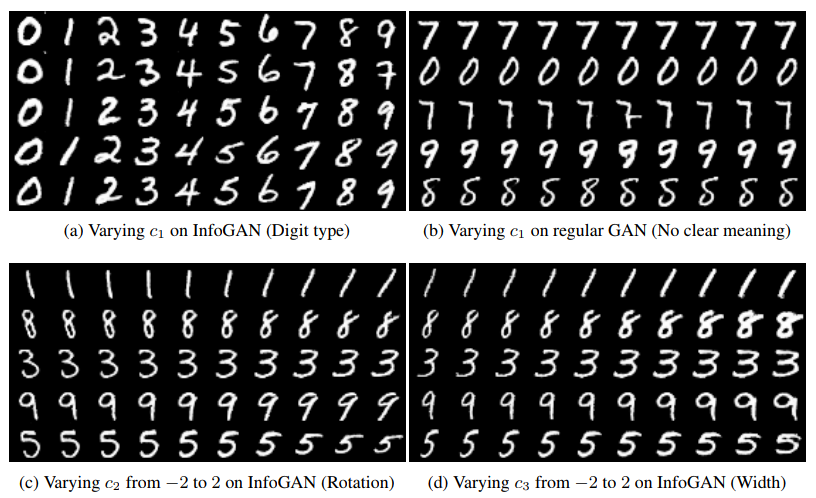
\includegraphics[width=\textwidth]{images/infogan-digits}
	\imgsrc{\cite{chen2016infogan}}
	\caption{\label{fig:infogan-digits} InfoGAN: Tweaking Latent Variables}
\end{figure}

However, this method does not provide a method of explicitly controlling the nature of the sampled data. Samples need to be generated first to understand which features have been represented in the additional latent variables.


\section{Controlled Generation of Text}

\cite{hu2017toward} use a variational autoencoder trained with the reconstruction objective and a KL-divergence minimization objective on the latent space with respect to a prior $p(z)$, as described in the original variational auto-encoding paper by \cite{kingma2013auto}. In addition to the reconstruction objective, the authors use additional discriminative training signals to adapt the desired attributes of the generated text. These training signals need to be propagated back to the encoder.

$x$ is the source corpus and the encoder is parameterized to generate a latent code $z$, which is a variational latent space that resembles a Gaussian prior. (This is enforced by a KL-divergence loss). The structured code $c$ is a known label of the text (discrete or continuous). The decoder generator produces the output corpus $\hat{x}$ conditioned on $(z, c)$. It uses greedy decoding, which predicts the word with maximal probability at each step \citep{langlais2007greedy}.

A classifier/regressor discriminator predicts the structured code of the output corpus $\hat{x}$ to ensure that it is the same as the one the generator was conditioned on i.e. $G(z, c)$. The discriminator is pre-trained.

Each decoder step in $\hat{x}$ is predicted using a softmax function scaled by a temperature $\tau$. Higher temperatures flatten the softmax distribution for each word prediction and increase word diversity. Conversely, setting $\tau = 0$ will resemble a discrete probability distribution over the corpus vocabulary. For their experiments, the authors gradually anneal $\tau \rightarrow 0$

The authors describe the following objectives to train their model:

\subsection{Variational Autoencoder}

A reconstruction loss that ensures that the generated sentence $\hat{x}$ is the same as the original sentence $x$. This is equivalent to minimizing the negative log-likelihood of generating $\hat{x}$. This is shown in Equation \ref{eqn:tcg-rec}
\begin{eqnarray} \label{eqn:tcg-rec}
	\mathcal{L}_{VAE}(\theta_G, \theta_E; x) &=& \nonumber
	- \mathbb{E}_{q_E(z|x)q_D(c|x)}[log p_G(x|z,c)] \\ & &
	+ KL(q_E(z|x)||p(z))
\end{eqnarray}


\subsection{Style Discriminator}

A discriminator validates if the predicted class/value for $\hat{x}$ is the same as the corresponding class/label for $x$. This is a cross-entropy loss over the probability distribution of the labels. This discriminator loss can be further subdivided into 2 terms, one that maximizes the log likelihood of predicting the correct class as in Equation \ref{eqn:tcg-disc-class}, and one that minimizes the empirically observed Shannon entropy of the predicted distribution, thereby incentivizing confident predictions, as in Equation \ref{eqn:tcg-disc-ent}.
\begin{equation} \label{eqn:tcg-disc-class}
	\mathcal{L}_s(\theta_D) = - \mathbb{E}_{X_L}[log q_D(c_L|x_L)]
\end{equation}
\begin{equation} \label{eqn:tcg-disc-ent}
	\mathcal{L}_u(\theta_D) = - \mathbb{E}_{p_G(\hat{x}|z,c)p(z)p(c)}
	[log q_D(c|\hat{x}) + \beta \mathcal{H}(q_D(c'|\hat{x}))]
\end{equation}


\subsection{Content Discriminator}

The encoder from loss equation \ref{eqn:tcg-rec}, is used to regenerate the latent distribution $z$ devoid of the structured code from the output distribution $\hat{x}$. The authors call this an \textbf{independence constraint}, in that regardless of the structured code $c$ that is currently present in either $x$ or $\hat{x}$, processing either through the generator should produce a consistent $z$. This allows the encoder to encode only latent factors that are independent of the structured code. This is shown in Equation \ref{eqn:tcg-ind-con}.
\begin{equation} \label{eqn:tcg-ind-con}
	\mathcal{L}_{attr, z}(\theta_G) = - \mathbb{E}_{p(z)p(c)}
	[log q_E(z|\tilde{G_{\tau}}(z,c))]
\end{equation}


They maximize the expected log likelihood of predicting the correct distribution of the structured code $c$ given the labelled examples $X_L$. This happens before the generator model training. They also maximize the expected log likelihood of predicting the correct distribution of the structured code $c$ given the generated sentences $\hat{x}$. Also minimize the empirically observed Shannon entropy of the observed discriminator prediction $q_D(c'|\hat{x})$, which reduces uncertainty and increases confidence of the structured code prediction. A wake-sleep algorithm \citep{hinton1995wake} is used to alternatively train the generator and discriminator.

The model was applied only to short sentences with length $<15$ words and the encoder-decoder setup is implemented using single layer LSTMs and the discriminator is implemented using a convolutional neural network (CNN). The KL loss weight is annealed from 0 to 1 during training.


\section{Aligned and Cross-Aligned Autoencoders}

\cite{shen2017style} aim to perform style transfer on language using non-parallel corpora by separating content from style. They re-align the latent spaces to perform three tasks: sentiment modification, decipherment of word-substitution ciphers, and recovery of word order. Their method involves learning an encoder that takes a sentence and its original style label as input, and maps it to a content representation devoid of style. This representation is then decoded by a decoder whose input is this encoded representation and the target style label.

There are two non-parallel corpora $X_1 = {x_1^{(1)} ... x_1^{(n)}}$, drawn from the prior $p(x_1|y_1)$ and $X_2 = {x_2^{(1)} ... x_2^{(n)}}$, drawn from the prior $p(x_2|y_2)$. The objective is to estimate the style transferred distributions $p(x_1|x_2;y_1,y2)$ and $p(x_2|x_1;y_1,y2)$.

The authors propose a constraint that $x_1$ and $x_2$'s marginal distributions can only be recovered if for any different styles $y, y' \in Y$, distributions $p(x|y)$ and $p(x|y')$ are different, which is a fair assumption to make because if $p(x|y)$ = $p(x|y')$, then the style changes would be indiscernible.

They also prove that if the content $z$ is sampled from a centred isotropic distribution, the styles cannot be recovered from $x$, but in the case of $z$ being a more complex distribution like a Gaussian mixture, then the affine transformation that converts $y, z$ into $x$ can be recovered.

The reconstruction loss is the same as the one used by a variation autoencoder for its reconstruction objective, as shown in Equation \ref{eqn:stca-rec}.
\begin{eqnarray} \label{eqn:stca-rec}
	\mathcal{L}(\theta_E,\theta_G)
	&=& \mathbb{E}_{x_1 \sim X_1}[-\log p_G(x_1|y_1,E(x_1, y_1))] \nonumber \\
	& & + \mathbb{E}_{x_2 \sim X_2}[-\log p_G(x_2|y_2,E(x_2, y_2))]
\end{eqnarray}

\subsection{Aligned Autoencoder}

The authors propose aligning the distributions $P_E(z|x_1)$ and $P_E(z|x_2)$ where $E$ is the encoder function. This is done by training an adversarial discriminator to distinguish between the two distributions.

The adversarial objective is expressed as below where $D(\cdot)$ predicts 0 if it predicts the source distribution to be $X_1$ and 1 if it predicts the source distribution to be $X_2$
\begin{eqnarray} \label{eqn:stca-align-adv}
	\mathcal{L}_{adv}(\theta_E,\theta_D)
	&=& \mathbb{E}_{x_1 \sim X_1}[-\log D(E(x_1,y_1))] \nonumber \\
	& & + \mathbb{E}_{x_2 \sim X_2}[-\log(1 - D(E(x_2,y_2)))]
\end{eqnarray}

The overall optimization objective combining equations \ref{eqn:stca-rec} and \ref{eqn:stca-align-adv} can be written as
\begin{equation}
	\mathcal{L} = \operatorname*{min}_{E,G} \operatorname*{max}_{D} \mathcal{L} - \lambda \mathcal{L}_{adv}
\end{equation}
where $\lambda$ is a balancing weight for the adversarial term.

\subsection{Cross-aligned Autoencoder}

This is similar to the aligned autoencoder approach, but instead of trying to align $P_E(z|x_1)$ and $P_E(z|x_2)$ using an adversarial discriminator, two distinct adversarial discriminators are used to align a sequence of real and transferred generator hidden states. i.e. $D_1$ is used to align the distributions $G(y_1, z_1)$ and $G(y_1, z_2)$. Similarly, $D_2$ is used to align the distributions $G(y_2, z_2)$ and $G(y_2, z_1)$. These discriminators are trained with the objective of being unable to identify the content distributions $P(z_1)$ and $P(z_2)$

Professor-forcing is used to train both of these discriminators. Professor forcing uses a discriminator to distinguish if the decoder hidden states are a result of training-time teacher forcing or test time scheduled sampling \citep{lamb2016professor}. This is a generalized version of simply using a final encoder state, as was the case in the Aligned Autoencoder solution.

The overall optimization objective combining equation \ref{eqn:stca-rec} and two discriminator variants of equation \ref{eqn:stca-align-adv} can be written as:
\begin{equation}
	\mathcal{L} = \operatorname*{min}_{E,G} \operatorname*{max}_{D} \mathcal{L} - \lambda (\mathcal{L}_{adv_1} + \mathcal{L}_{adv_2})
\end{equation}

As opposed to the simple feed-forward classifier used in the aligned autoencoder, the cross-aligned autoencoder uses convolutional nets for text classification. They use Yelp reviews as the data set with rating $>3$ as positive and rating $<3$ as negative examples. Reviews with a sentence count $>10$ and sentences with a word count $>10$ are filtered out. The vocabulary size used is $10K$. Style transfer is evaluated using a pre-trained classifier. Language fluency and content preservation was evaluated using human assessments.

\section{Style Embedding Autoencoder}

\cite{fu2017style} employ two distinct models to perform style transfer
\begin{itemize}
	\item A \textbf{multi-decoder model} that use the distinct decoders to produce text in different styles. This implicitly means that the number of decoders that need to be trained scales with the number of distinct label values to train.
	\item A \textbf{style-embedding model} with a single decoder that generate text in different styles. This method utilizes a separate style embedding matrix, of size $n * m$ where $n$ is the number of distinct label values and $m$ is an arbitrarily chosen embedding size.
\end{itemize}

In contrast with the previous models described, this work uses a deterministic autoencoder in lieu of a variational autoencoder. For our purposes, we focus on the style-embedding model, since it requires explicit disentanglement and uses fewer model parameters for each label addition, compared to the multi-decoder model.

The training objectives used for this model include the reconstruction objective for the autoencoder, the style label discriminative objective for a classifier on the latent space, and the adversarial loss propagated back to the autoencoder from the representation learned in the content space.

The autoencoder is trained to product only the salient features that represent the content of the sentences i.e. the content space, and the style embedding vector is trained via back-propagation of the reconstruction loss.

The reconstruction loss is the same as that of a standard deterministic autoencoder.
\begin{equation}
	\mathcal{L}_{seq2seq} = -\sum_{i=1}^M \log P(\hat{x}_i|x_i;\theta_e;\theta_d)
\end{equation}
where $M$ is the number of training examples and $\theta_e$ and $\theta_d$ are the encoder and decoder parameters respectively.

A discriminative classifier is trained on the latent content space learned by the autoencoder, to distinguish between the different possible styles.
\begin{equation}
	\mathcal{L}_{disc} = -\sum_{i=1}^M \log P(l_i|Encoder(x_i;\theta_e);\theta_c)
\end{equation}
where $M$ is the number of training examples and $\theta_e$ and $\theta_c$ are the encoder and discriminative classifier parameters respectively.

An adversarial objective is applied to the content representation. This objective aims to maximize entropy of the predicted label from the content representation by minimizing the following objective:
\begin{equation}
	\mathcal{L}_{adv} = -\sum_{i=1}^M\sum_{j=1}^N \mathcal{H}(P(j|Encoder(x_i; \theta_e); \theta_c))
\end{equation}
where $M$ is the size of the training data and $N$ is the number of distinct styles. Using this adversarial entropy objective, the encoder is penalized and therefore trained to produce a latent content representation which is independent of style.

Similar to the persona-based neural conversation model \citep{li2016persona}, a style embedding is learned for each different style. The conditional generation is done using recurrent neural networks with the inputs being the recurrent networks current state, and the style embedding to apply.

The style embeddings matrix is not directly parameterized by the encoder, but the learning algorithm propagates changes based on how well it combines with the content representation to reconstruct the original text.

The methods are evaluated in the following manner:
\begin{itemize}
	\item Transfer strength is evaluated using a simple classifier
	\item Content preservation is evaluated by computing the cosine distance between the original and the generated text embeddings.
\end{itemize}


Several other works have also been published in this domain recently including: using cyclical translation to strip style as a pre-processing step, followed by a multi-decoder model to generate style-transferred sentences \citep{prabhumoye2018style}, conditioned RNN decoding with a set of tunable attributes \citep{ficler2017controlling}, using maximum-mean discrepancy metrics to separate common and discriminative factors in distinct source corpora \citep{larsson2017disentangled} etc.


In the next chapter we describe the method used to learn attribute disentangled representations and provide details of the necessary objective and regularizations used in the our model.


%======================================================================
\chapter{Challenges}
%======================================================================

\todo[inline]{Merge the contents of this chapter into other chapters}

\section{Non-interpretable Latent Representations}

The randomness and inscrutability of the learning processes in neural networks has prompted research into learning interpretable representations \citep{chen2016infogan}.

Although neural networks have proved to be highly capable function approximators in the general machine intelligence literature over the past couple of decades, without any explicit additional modelling, the weights of a neural network are learnt in an arbitrary manner to approximate a function modelled by a user-defined loss variable.

Due to this non-explainability of the weights of neural networks, they have been used as a black-box in practice, and the non-explainability hampers their adoption in use-cases required explicit audits and accountability, and for humans to reason about why a system chose a particular outcome over the other options available.

We believe that the disentanglement of the learned weights of a neural network are an important step in the direction of addressing this shortcoming, using available labels to force representation learning to adhere to a pre-defined separation scheme in the latent space.


\section{Quantitative Evaluation of Language Quality}

The evaluation of novel generated text to measure its perceived quality, naturalness, fluency and compliance with predefined attributes, like sentiment, tense etc.

For the presence of a certain attribute, it is fairly simple to devise a classification model that is trained on a large corpora of samples labelled as such.

However it is much more difficult to unambiguously state what makes a body of text more fluent or natural that another with mathematical rigour using quantitative metrics.

To offset this problem while stilling avoiding the need for human annotators to evaluate the target text, we have utilized techniques like sentences embedding similarity, augmented by the removal of words that highly correlate with any specific label, as proposed by the previous work by \cite{fu2017style}. This is described further in section \ref{ssec:content-preservation-metric} of the Experiments chapter.


%======================================================================
\chapter{Approach}
%======================================================================

We provide a novel approach to solve this open problem, and juxtaposes this approach and its experimental results against the current state-of-the-art models. We empirically demonstrate the separation of content and style spaces by demonstrating the inferred spaces of labelled sentences in a sentiment-transfer task, where the positive sentences in the test set are converted to equivalent sentences with a negative sentiment, and vice-versa.

This model is also generalizable using its standard implementation to problems involving multiple classes, like style transfer by authors, artists, topic etc.

Our model is built upon an autoencoder with a sequence-to-sequence (Seq2Seq) neural network \citep{sutskever2014sequence}, as described in Section \ref{ssec:seq2seq-objective}. This is the primary objective of the algorithm, whose objective function is to simply reconstruct the input text. We implement our model with both deterministic autoencoders \citep{baldi2012autoencoders} as well as variational autoencoders \citep{kingma2013auto}.

Then we introduce two auxiliary losses, multi-task loss and adversarial loss in Sections \ref{ssec:multitask-objective} and \ref{ssec:adversarial-style-objective}, respectively. In addition to these auxiliary losses, we propose a novel bag-of-words adversarial loss in Section \ref{ssec:adversarial-bow-objective}. This makes our model a dual-adversary model. Section \ref{ssec:generating-novel-text} presents the approach to transfer style in natural language generation.

Figures \ref{fig:model-overview-training} and \ref{fig:model-overview-inference} depict the training and generation processes of our approach.

\begin{figure}[ht]
	\centering
	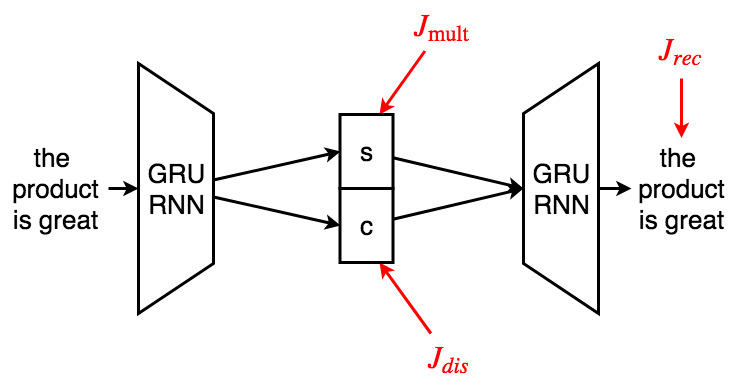
\includegraphics[width=\linewidth]{images/model-overview-training}
	\caption{Overview of Model Training}
	\label{fig:model-overview-training}
\end{figure}

\begin{figure}[ht]
	\centering
	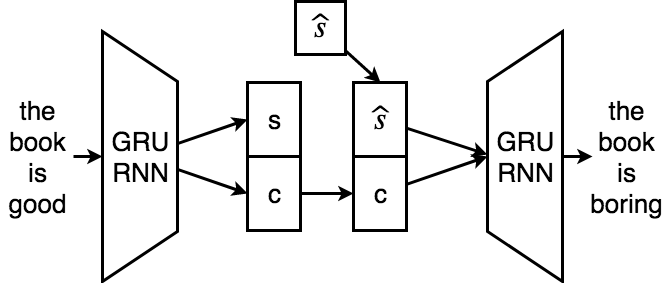
\includegraphics[width=\linewidth]{images/model-overview-inference}
	\caption{Overview of Model Inference}
	\label{fig:model-overview-inference}
\end{figure}


\section{Autoencoder} \label{ssec:seq2seq-objective}

An autoencoder encodes an input to a latent vector space, from which it decodes the input itself. By doing so, the autoencoder learns meaningful representations of data. This serves as our primary learning objective. Besides, we also use the autoencoder weights  for text generation in the attribute style-transfer application.

Let $x=(x_1, x_2, \cdots x_n)$ be an input sentence. The encoder encodes $x$ by a recurrent neural network (RNN) with gated recurrent units (GRU) \citep{cho2014learning}, and obtains a hidden state $\bm h$, which in our formulation, is two separate spaces, $\bm s$ for style and, $\bm c$ for content, which still requires an equivalent number of parameters compared to a vanilla RNN encoder.

Then a decoder RNN generates a sentence, which ideally should be $x$ itself. Suppose at a time step $t$, the decoder RNN predicts the word $x_t$ with probability $p(x_t | \bm h, x_1 \cdots x_{t-1})$, then the autoencoder is trained with cross-entropy loss, given by

First the encoder produces the style and content, given that $\theta_{E_s}$ represents the subset of encoder parameters responsible for the production of the style vector and $\theta_{E_c}$, similarly, represents the encoder responsible for the production of the content vector.
\begin{eqnarray*}
	\bm s &=& \theta_{E_s}(x) \nonumber \\
	\bm c &=& \theta_{E_c}(x) \nonumber
\end{eqnarray*}

Following which the decoder attempts to predict the original distribution of $x$ by predicting the softmax over the vocabulary size, for as many time steps as the sequence length, as shown in Equation \ref{eqn:dae-rec}
\begin{equation} \label{eqn:dae-rec}
	\mathcal{L}_\text{rec}(\bm\theta_E,\bm\theta_D)= -\mathbb{E}[log p_D(x|\bm s, \bm c)]
\end{equation}
where $\bm\theta_E$ and $\bm\theta_D$ are the parameters of the encoder and decoder, respectively.

Since this loss trains the autoencoder to reconstruct $x$, it is also called the reconstruction loss.


\subsection{Variational Autoencoder}

In addition to the deterministic auto-encoding objective presented above, we also implement a variational autoencoder. The variational sampling and KL-divergence losses are applied for both the style space $\bm s$ and the content space $\bm c$. The weights applied to each KL-divergence loss is tuned independently as a hyperparameter.

Equation \ref{eqn:vae-rec} shows the reconstruction objective that is minimized by the model in the VAE variant of our model.

\begin{eqnarray} \label{eqn:vae-rec}
	\mathcal{L}_\text{rec}(\theta_D, \theta_E; x) &=& \nonumber
	- \mathbb{E}_{q_{E_s}(\bm s|x) q_{E_c}(\bm c|x)} [log p_D(x|\bm s, \bm c)] \nonumber \\ & &
	+ \lambda_{\text{skl}} KL(q_{E_s}(\bm s|x)||p(z)) \nonumber \\ & &
	+ \lambda_{\text{ckl}} KL(q_{E_c}(\bm c|x)||p(z))
\end{eqnarray}

The motivation for using a variational autoencoder variant to compare the base deterministic autoencoder model to, is the property of VAEs to learn smooth and continuous latent spaces, without many dead zones in the latent space that cannot be sampled from. \cite{bowman2016generating} show this empirically by using the latent space of a text variational autoencoder to interpolate between and generate novel sentences from the latent spaces between two valid sentences from a corpus.

Since our objective is to use empirically inferred latent vectors to eventually achieve the attribute style transfer objective, it would be beneficial to juxtapose the experimental performance of a variational autoencoder against a deterministic autoencoder.


Besides the above reconstruction losses, we design auxiliary losses to disentangle the latent space such that $\bm h$ can be separated into two spaces $\bm s$ and $\bm c$, representing style and content respectively, i.e., $\bm h = [\bm s ; \bm c]$, where $[\cdot;\cdot]$ denotes concatenation. We also design additional regularizations on the latent space to encourage learning this disentangled representation.


\section{Multi-Task Loss} \label{ssec:multitask-objective}

Our first auxiliary loss ensures the style space does contain style information. We build a classifier trained using the style space $\bm s$ as its features, predicting the style label $y$, which is a part of the training data.

This loss can be viewed as a multi-task objective, in addition to the original reconstruction objective, which ensures that the neural network not only decodes the sentence, but also predicts its sentiment from a sub-space of the latent representation. Similar multi-task losses have been used in previous work for sequence-to-sequence learning \citep{luong2015multi}, sentence representation learning \citep{jernite2017discourse} and sentiment analysis \citep{balikas2017multitask}, among others.

In our application, we follow previous work \citep{hu2017toward,shen2017style,fu2017style} and treat the sentiment as the style of interest for our primary evaluation. However, since our model generalizes to more that one class, we uses a simple multi-layer perceptron (MLP) followed by a softmax distribution over the possible labels. The softmax function can be expressed as the following expression
\begin{equation*}
	\sigma(\mathbf{z})_j = \frac{e^{z_j}}{\sum_{k=1}^K e^{z_k}} \text{for} j \in {1, \cdots K}
\end{equation*}
where $z_j$ denotes an arbitrary label's unweighted probability and $K$ is the total number of labels in the training data. The softmax distribution is re-weighted such that it's constituent values sum up to 1, which is very useful to model probability predictions over an arbitrary number of classes.

The discriminative classification predicted distribution is given by
\begin{equation} \label{eqn:class-pred}
	p(y | \bm s; \bm\theta_\text{mult}) = softmax(\bm w_\text{mult}^\top \bm s + b_\text{mult})
\end{equation}
where $\bm\theta_\text{mult}=[\bm w_\text{mult}; b_\text{mult}]$ are the classifier's parameters for multi-task learning.

This is trained using a simple cross-entropy loss.
\begin{equation} \label{eqn:multi-task-loss}
	\mathcal{L}_\text{mult}(\bm\theta_{E};\bm\theta_\text{mult}) =
	\mathbb{E}_{y'} [\log p(y | \bm s; \bm\theta_\text{mult})]
\end{equation}
where $\bm\theta_E$ are the encoder's parameters and $y'$ is the true class distribution.


\section{Adversarial Style Discriminator} \label{ssec:adversarial-style-objective}

The above multi-task loss only operates on the style space, but does not have an effect on the content space $\bm c$. With only the multi-task loss, we cannot guarantee that the encoder would not choose to encode stylistic features within the content space.

We therefore apply an adversarial loss to disentangle the content space from style information, inspired by adversarial generation \citep{goodfellow2014generative}, adversarial domain adaptation \citep{liu2017adversarial}, and adversarial style transfer \citep{fu2017style}.

The idea of adversarial loss is to introduce an adversary that deliberately attempts to discriminate style $s$ of training samples using only the content vector $\bm c$. Then the autoencoder is trained to learn such a content vector space that its adversary cannot predict style information.

Concretely, the adversarial discriminator predicts style $y$ by using a softmax distribution over a multi-layer perceptron
\begin{equation}
	p(y | \bm c; \bm\theta_\text{dis}) = softmax(\bm w_\text{dis}^\top \bm c + b_\text{dis})
\end{equation}
where $\bm\theta_\text{dis}=[\bm w_\text{dis}; b_\text{dis}]$ are the parameters of the adversary.

It is trained by minimizing the following objective
\begin{equation} \label{eqn:adv-disc-loss}
	\mathcal{L}_\text{dis}(\bm\theta_{E};\bm\theta_\text{dis}) =
	\mathbb{E}_{y'} [\log p(y | \bm c; \bm\theta_\text{dis})]
\end{equation}

The adversarial loss appears similar to the multi-task loss as in Equation \ref{eqn:multi-task-loss}. However, it should be emphasized that, for the adversary, the gradient is not propagated back to the autoencoder, i.e., $\bm c$ is treated as shallow features. The only adversarial component is the loss itself. The network parameters are mutually exclusive for the autoencoder and the adversarial discriminator.

Having trained an adversary, we would like the autoencoder to learn latent representations, that $\bm c$ is not discriminative in term of the style or attribute we want to transfer. In other words, we penalize the entropy of the adversary's prediction, given by
\begin{equation}
	\mathcal{L}_\text{adv}(\bm\theta_E) = \mathcal{H}(p_\text{dis}(y | \bm c))
\end{equation}
where $\mathcal{H}=-\sum_{i\in\text{labels}} p_i\log p_i$ is the empirical Shannon entropy of the distribution. The adversarial objective is maximized, in this phase, with respect to the encoder. The motivation behind this objective is to increase the uncertainty of the discriminative classifier with respect to predicting style from the content vector. The maximum entropy value attainable over the distribution of attributes is the point at which each label is predicted with equal-probability i.e. the highest uncertainty.


\section{Adversarial Bag-of-Words Discriminator} \label{ssec:adversarial-bow-objective}

In addition to the auxiliary losses used above, we also propose a novel bag-of-words discriminator on the style space. The motivation for having this objective is to try and emulate the adversarial signal provided by the style discriminator, but and do the same for the content. Here, we define the content of the sentence as the words from the original sentence without any sentiment words.hu2004mining
hu2004mining
The input sentences $x$ are represented as a vector of the same size as the corpus vocabulary, with each index of the vector a discrete probability of a word's presence in the sentence. Therefore, this bag-of-words representation is comprised of only 1s and 0s.

The bag-of-words discriminator, uses the style vector produced by the autoencoder model and tries to predict the true bag-of-words distribution using a set of parameters that are distinct from those of the autoencoder. The discriminator uses a logistic regression to predict a probability of each words occurrence in the original sentence, between 0 and 1.
\begin{equation}
	p(b | \bm s; \bm\theta_\text{bow}) = \sigma(\bm w_\text{bow}^\top \bm s + b_\text{bow})
\end{equation}
where $b$ is the predicted bag-of-words distribution.

This objective is trained in a similar method to the style adversary, by using a cross-entropy loss
\begin{equation} \label{eqn:adv-bow-disc-loss}
	\mathcal{L}_\text{bow}(\bm\theta_{E};\bm\theta_\text{bow}) =
	\mathbb{E}_{b'} [\log p(b | \bm c; \bm\theta_\text{bow})]
\end{equation}
where $b'$ is the true distribution and can be considered part of the training data.

Similar to the style adversary, the empirical Shannon entropy of the predicted distribution is provided as a training signal for the autoencoder model to maximize.
\begin{equation}
	\mathcal{L}_\text{badv}(\bm\theta_E) = \mathcal{H}(p_\text{bow}(b | \bm s))
\end{equation}

The motivation for this adversarial loss is similar to the one used in the context of the style discriminator. We want to encourage the encoder to learn a representation of style that the bag-of-words discriminator cannot predict most of the original words from.

\subsection{Lexicon Augmented Discriminator}

An improvement to the bag-of-words discriminator could be made assuming the availability of a lexicon of words that are associated with a high probability with each of the styles that we are trying to disentangle.

The bag-of-words representation that excludes these words can now be created, such that the size of each representation is $(\text{\# vocab words}) \setminus (\text{\# lexicon words})$.

The bag-of-words adversary will not penalize the autoencoder model for encoding words that are pertinent and discriminative for style that may be encoded in the style space. For the sentiment task in our experiments, we use a lexicon of positive and negative sentiments words curated by \cite{hu2004mining}.


\section{Style Dropout Regularization} \label{ssec:style-dropout}

In addition to the regular training objectives, we also describe a novel regularization technique for disentanglement tasks. This method can also be viewed as analogous to a training objective like the bag-of-words loss.

In our formulation of the model, we describe the main adversarial loss for style disentanglement by training a discriminator on the content space. However, there is a possibility of the autoencoder learning to ignore the content vector during generation entirely and use only the style space for encoding and later decoding the salient features of the corpus. This scenario is depicted in \ref{fig:model-content-bypass} and can be thought of as the model bypassing the content space due to the presence of an adversary that penalizes any signals for style.

\begin{figure}[ht]
	\centering
	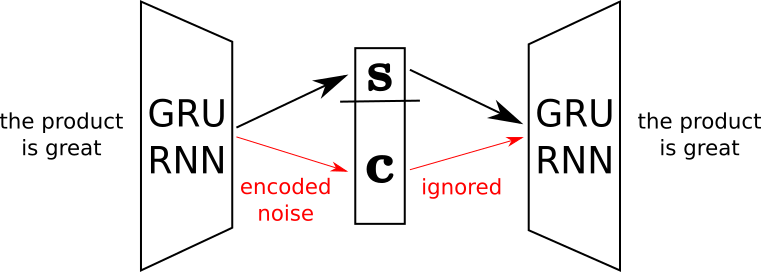
\includegraphics[width=\linewidth]{images/model-content-bypass}
	\caption{Content Space Bypassing}
	\label{fig:model-content-bypass}
\end{figure}

To address this issue, we propose a customized version of Dropout \cite{srivastava2014dropout}. Similar to how each neuron in a network is dropped out with a pre-defined probability in the general version of dropout, in this version, we drop out entire style vectors in the mini-batch randomly with a pre-defined probability. The motivation for doing this is to reinforce the fact that the content latent vector is not to ignored for the auto-encoding task despite the negative training signal from the adversary.


\section{Training Process}

The overall loss used for the autoencoder is thus comprised of four different, objectives, the reconstruction objective, the multi-task objective and the style and content adversaries.
\begin{eqnarray*}
	\mathcal{L}_\text{ovr} &=&
	\mathcal{L}_\text{rec}(\bm\theta_E, \bm\theta_D)
	+ \lambda_\text{mult} \mathcal{L}_\text{mult} (\bm\theta_E,\bm\theta_\text{mult}) \\ & &
	- \lambda_\text{adv} \mathcal{L}_\text{adv}(\theta_E)
	- \lambda_\text{badv} \mathcal{L}_\text{badv}(\theta_E)
\end{eqnarray*}
where $\lambda_\text{mult}$, $\lambda_\text{adv}$ and $\lambda_\text{badv}$ balance these losses.

To summarize the model training setup, our training process is a loop of the minimization objectives described in Algorithm \ref{alg:training-process}.

\begin{algorithm}[H]
	\While{epochs remaining}{
		minimize $\mathcal{L}_\text{dis}(\bm\theta_\text{dis})$ w.r.t. $\bm\theta_\text{dis}$\;
		minimize $\mathcal{L}_\text{bow}(\bm\theta_\text{bow})$ w.r.t. $\bm\theta_\text{bow}$\;
		minimize $\mathcal{L}_\text{ovr}(\bm\theta_E, \bm\theta_D)$ w.r.t. $\bm\theta_E, \bm\theta_D, \bm\theta_\text{mult}$\;
	}
	\caption{\label{alg:training-process} Training Algorithm}
\end{algorithm}


\section{Generating Style-Transferred Sentences} \label{ssec:generating-novel-text}

A direct application of our disentangled latent space is style transfer for natural language generation. For example, we can generate a sentence with generally the same meaning (content) but an opposite sentiment.

Let $x$ be an input sentence with $\bm s$ and $\bm c$ being the encoded, disentangled style and content vectors, respectively. If we would like to transfer its content to a different style, we compute an empirical estimate of the target style's vector $\hat{\bm s}$ by
$$\hat{\bm s}=\frac{\sum_{i\in\text{target style}}\bm s_i}{\text{\# target style samples}}$$. The inferred target style $\hat{\bm s}$ is concatenated with the encoded content $\bm c$ for decoding (Figure \ref{fig:model-overview-inference}).


\subsection{Nearest-Neighbour Approach for Sentence Generation} \label{ssec:nearest-neighbour-inference}

The inference approach described above using the empirically learned mean embedding in the style space and applies it to all future inference requirements. Though simple and intuitive, this method is fairly rigid and doesn't take into account the fact that the inference time sentences' content could vary from the acceptable content embeddings that can be coupled with the mean style embedding used.

To address this, we also propose a nearest neighbour approach to identify better candidates for the style embedding than the empirical mean of training time style embeddings. Algorithm \ref{alg:nearest-neighbour} describes our method.

\begin{algorithm}[H]
	\KwData{$S \Rightarrow$ empirical style embeddings from the training data}
	\KwData{$C \Rightarrow$ empirical content embeddings from the training data}
	\KwData{$s \Rightarrow$ inferred content embedding (singular) of a test sample}
	\KwData{$c \Rightarrow$ inferred style embedding (singular) of a test sample}
	\KwData{$N \Rightarrow$ number of neighbours (hyperparameter)}
	\KwResult{new sentence generation style vector for transferring style}
	$(S, C) \Rightarrow$ pairs of (style, content) embeddings\;
	$(\text{cosine-distance}, \text{style-vector}) \Rightarrow$ empty list of tuples\;
	\For{$s_t, c_t$ in $(S, C)$}{
		Compute $cd$, the cosine distance between $c$ and $c_t$\;
		Add tuple $(cd,s_t)$ to $(\text{cosine-distance}, \text{style-vector})$\;
	}
	$\text{best-tuples} \Rightarrow$ N best tuples with minimum cosine distance in $(\text{cosine-distance}, \text{style-vector})$\;
	define $\text{aggregate-style-vector}$\;
	\For{$cd, s_t$ in $\text{best-tuples}$}{
		Add $s_t$ to $\text{aggregate-style-vector}$\;
	}
	\KwRet{$\frac{\text{aggregate-style-vector}}{N}$}\;

	\caption{\label{alg:nearest-neighbour} Nearest-Neighbour Algorithm}
\end{algorithm}

However, this method is computationally more expensive since, for each test sentence, we need to iterate over the empirical content embeddings whose number is of the same order of magnitude as the training data.


%======================================================================
\chapter{Experiments}
%======================================================================

\section{Dataset and Task}

We conduct experiments on two datasets, the details for which are given below.

\subsection{Yelp Service Reviews}

The model is tested on a subset of the Yelp review dataset \citep{challenge2013yelp} and has been sourced from the code repository accompanying the implementation of the paper by \cite{shen2017style} open-sourced by the authors~\footnote{\url{https://github.com/shentianxiao/language-style-transfer}}. It contains 444101, 126670 and 63483 sentences for train, validation, and test, respectively, each sampling accompanied by binary sentiment labels. The maximum sentence length is 15, and the vocabulary size is about 9200.

\subsection{Amazon Product Reviews}

The model is trained and tested on an Amazon product reviews data-set~\footnote{\url{http://jmcauley.ucsd.edu/data/amazon/}}, following \cite{fu2017style}. The reviews were sourced from the code repository accompanying the paper~\footnote{\url{https://github.com/fuzhenxin/text_style_transfer}}. It contains 559142, 2000, 2000 sentences for train, validation, and test, respectively, each sampling accompanied by binary sentiment labels. The maximum sentence length is 20, and the vocabulary size is about 58000.


\section{Implementation Details and Model Hyper-parameters}

We implement the model in Tensorflow \citep{abadi2016tensorflow}, and utilize Scikit-learn \cite{pedregosa2011scikit} for latent-space classification evaluation metrics.

One of the most challenging aspects of training a variational autoencoder (VAE) is avoiding posterior collapse. In previous work \citep{yang2017improved, bowman2016generating, bahuleyan2017variational}, this has been done using manually crafted annealing schedules for weight of the KL-divergence term. We utilize the $\tanh$ annealing schedule proposed by \cite{bahuleyan2017variational}, and also use their technique of appending the latent vector ($[\bm s; \bm c]$) to the hidden state of the recurrent decoder at each time-step of decoding. Greedy decoding is utilized to predict the next word at each time-step.

The model uses style embeddings of size $8$ and content embeddings of size $128$ by default. The remaining hyper-parameters are shared as part of the default configuration in the code repository \footnote{\url{https://github.com/vineetjohn/linguistic-style-transfer}}.


\section{Evaluation Metrics} \label{sec:evaluation-metrics}

\subsection{Transfer Strength}

Transfer strength can be defined as a measure of how successful the model has been in generating sentences that are consistent with the attribute the needs to be transferred into them. This can be formulated as a Natural Language Understanding (NLU) task that takes in a sentence as input and predicts the presence of an attribute that we train the model to transfer.

Consistent with the approach taken in \cite{hu2017toward}, \cite{shen2017style} and \cite{fu2017style}, we train a separate model that learns to predict the class among the different classes to which transfer is possible. We use an open source implementation of the work presented by \cite{kim2014convolutional}, which is a convolutional neural network (CNN) model used for text classification, and build it into our model using an open-source implementation as a reference~\footnote{\url{https://github.com/dennybritz/cnn-text-classification-tf}}. This model has frequently been used as a text classification baseline to compare against \citep{tai2015improved} \citep{kiros2015skip} \citep{zhang2015character}.

This CNN classifier is trained on the entire corpus described in the previous section, with a held out validation set to assess improvements in accuracy over time. The test set for this classifier are the style-transferred sentences generated from the autoencoder model.

The style transfer strength is the ratio of sentences successfully transferred to the target style, to the total number of test sentences.
\begin{equation*}
	\text{transfer-strength} = \frac{count(\text{generated sentences with target style attribute})}{count(\text{generated sentences})}
\end{equation*}

Therefore, the optimal style transfer strength score is 1 and the worst is 0. Here, we choose to ignore the classification errors by our automated classification model, since a good model (with a high classification accuracy) would mis-classify approximately equal samples in each label, and a biased classifier would negatively impact the style transfer strength score.

The classifier we train achieves a classification accuracy of approximately 0.97 on the validation set used while training.

\subsection{Content Preservation} \label{ssec:content-preservation-metric}

The content preservation metric used by \cite{fu2017style} is also used in our work to judge content preservation of the generated sentences compared to the original. This metric is needed to ensure that the generated sentence doesn't talk about content, subjects or topics entirely different compared to the original sentence.

This method uses 100-dimensional GloVe embeddings \citep{pennington2014glove} pre-trained on the Wikipedia + GigaWord corpora~\footnote{\url{https://nlp.stanford.edu/projects/glove/}}. The min, mean and max GloVe word embeddings for each sentence are concatenated together to create a sentence representation. The cosine similarity between the source sentence and target sentence is used as a measure of content preservation.

Let $W$ be the set of word embeddings in a sentence $s$. Then the sentence embedding would be given by
\begin{equation*}
	\text{sentence-embedding} = [min(W);max(W);mean(W)]
\end{equation*}

Then the cosine similarity between two sentences $s_1$ and $s_2$ is obtained by
\begin{equation*}
	\text{cosine-similarity} = 1 - \cos(\text{sentence-embedding}_1, \text{sentence-embedding}_2)
\end{equation*}
where $\text{sentence-embedding}_1$ and $\text{sentence-embedding}_2$ are the sentence embeddings for $s_1$ and $s_2$ respectively. The mean cosine similarity of all the sentences in the test set is the content preservation that is reported for the experiment.

\begin{table}[ht]
	\centering
	\begin{tabular}{| p{0.45\linewidth} | p{0.45\linewidth} |}
		\hline
		\textbf{{Original (Positive)}}                                                      & \textbf{Transferred (Negative)}                  \\
		\hline
		\hline
		we had the shrimp with vegetables and shrimp fried rice both lovely                 & we had the bacon cheeseburger and it was cold    \\
		\hline
		both dishes prepared with quality veggies                                           & eggs benedict with no flavor                     \\
		\hline
		my appetizer was also very good and unique                                          & my steak was very dry and flavorless             \\
		\hline
		both times i have eaten the lunch buffet and it was outstanding                     & yes i have had the worst pizza i have ever had   \\
		\hline
		the new york eggrolls are outstanding and the beef dishes we ordered were flavorful & the main issue was our server was extremely rude \\
		\hline
	\end{tabular}
	\\
	\begin{tabular}{| p{0.45\linewidth} | p{0.45\linewidth} |}
		\hline
		\textbf{{Original (Negative)}}                                        & \textbf{Transferred (Positive)}        \\
		\hline
		\hline
		the chicken '' strip were paper thin oddly flavored strips            & the bread was wonderful as well        \\
		\hline
		the big chicken sandwich should be called the big mayonnaise sandwich & the salsa is the best i have ever had  \\
		\hline
		fries are not worth coming back                                       & prices are good                        \\
		\hline
		but honestly the worst hookah in las vegas                            & very authentic food in the east valley \\
		\hline
		second the service was terribly slow                                  & the sushi was delicious                \\
		\hline
	\end{tabular}
	\caption{Examples of poor content preservation while transferring sentiment}
	\label{tab:poor-content-preservation}
\end{table}

As seen in the examples above, it is easy to optimize for a style-transfer objective as long as there are no constraints on the content preservation regularization. To ensure this does not happen, we typically use a much larger content latent space than style latent space, as well as add the necessary regularizations discussed in the previous chapter.

Similar to \cite{fu2017style}, for the sentiment task, we exclude words from a sentiment lexicon \citep{hu2004mining} while evaluating the content preservation score.

However, a drawback of this content preservation metric devised by \cite{fu2017style} is that it can take a smaller range of possible values. The maximum content preservation value achievable is 1, but from empirical experiments performed by matching random pairs of sentences, the content preservation is $0.7591 \pm 0.0004$. This can be treated as an approximate lower bound on the metric for model assessment.

\subsection{Word Overlap}

In addition to the content preservation metric described above, we also utilize a simpler unigram overlap metric. Given a source sentence $x$ and a attribute style transferred sentence $y$, let $w_x$ and $w_y$ be the set of unique words present in $x$ and $y$ respectively. Then, the word overlap score can be calculated using
\begin{equation*}
	\text{word-overlap} = \frac{count(w_x \cap w_y)}{count(w_x \cup w_y)}
\end{equation*}
which is simply a normalized measure of overlapping unigrams in the source and target.

Theoretically, the word overlap score ranges from 0 to 1. However, in practice, since the expectation is that some words will be changed due to the style-transfer process, we wish to strike a good-balance with respect to the style transfer strength and original content preservation. Using experiments on random pairs of sentences, the word overlap score computed is $0.0098 \pm 0.0006$, which can again, be treated as a more realistic approximate lower-bound on this metric.

Word overlap can be used interchangeably with the 'Content Preservation' metric described above. For the experiments in this work, we report both.

\subsection{A note about Cycle Consistency Loss}

The cycle consistency loss is described in the image domain-adaptation work done by \cite{zhu2017unpaired}. Given domains $X$ and $Y$, They aim to learn a mapping similar to ours, $G: X \rightarrow Y$ which transfers attributes of $X$ to $Y$. At the same time, they also learn an inverse mapping $F: Y \rightarrow X$. The cycle consistency loss is the step that pushes $F(G(X)) \approx X$ and $G(F(Y)) \approx Y$, as shown in Figure \ref{fig:cycle-consistency}.

\begin{figure}[ht]
	\centering
	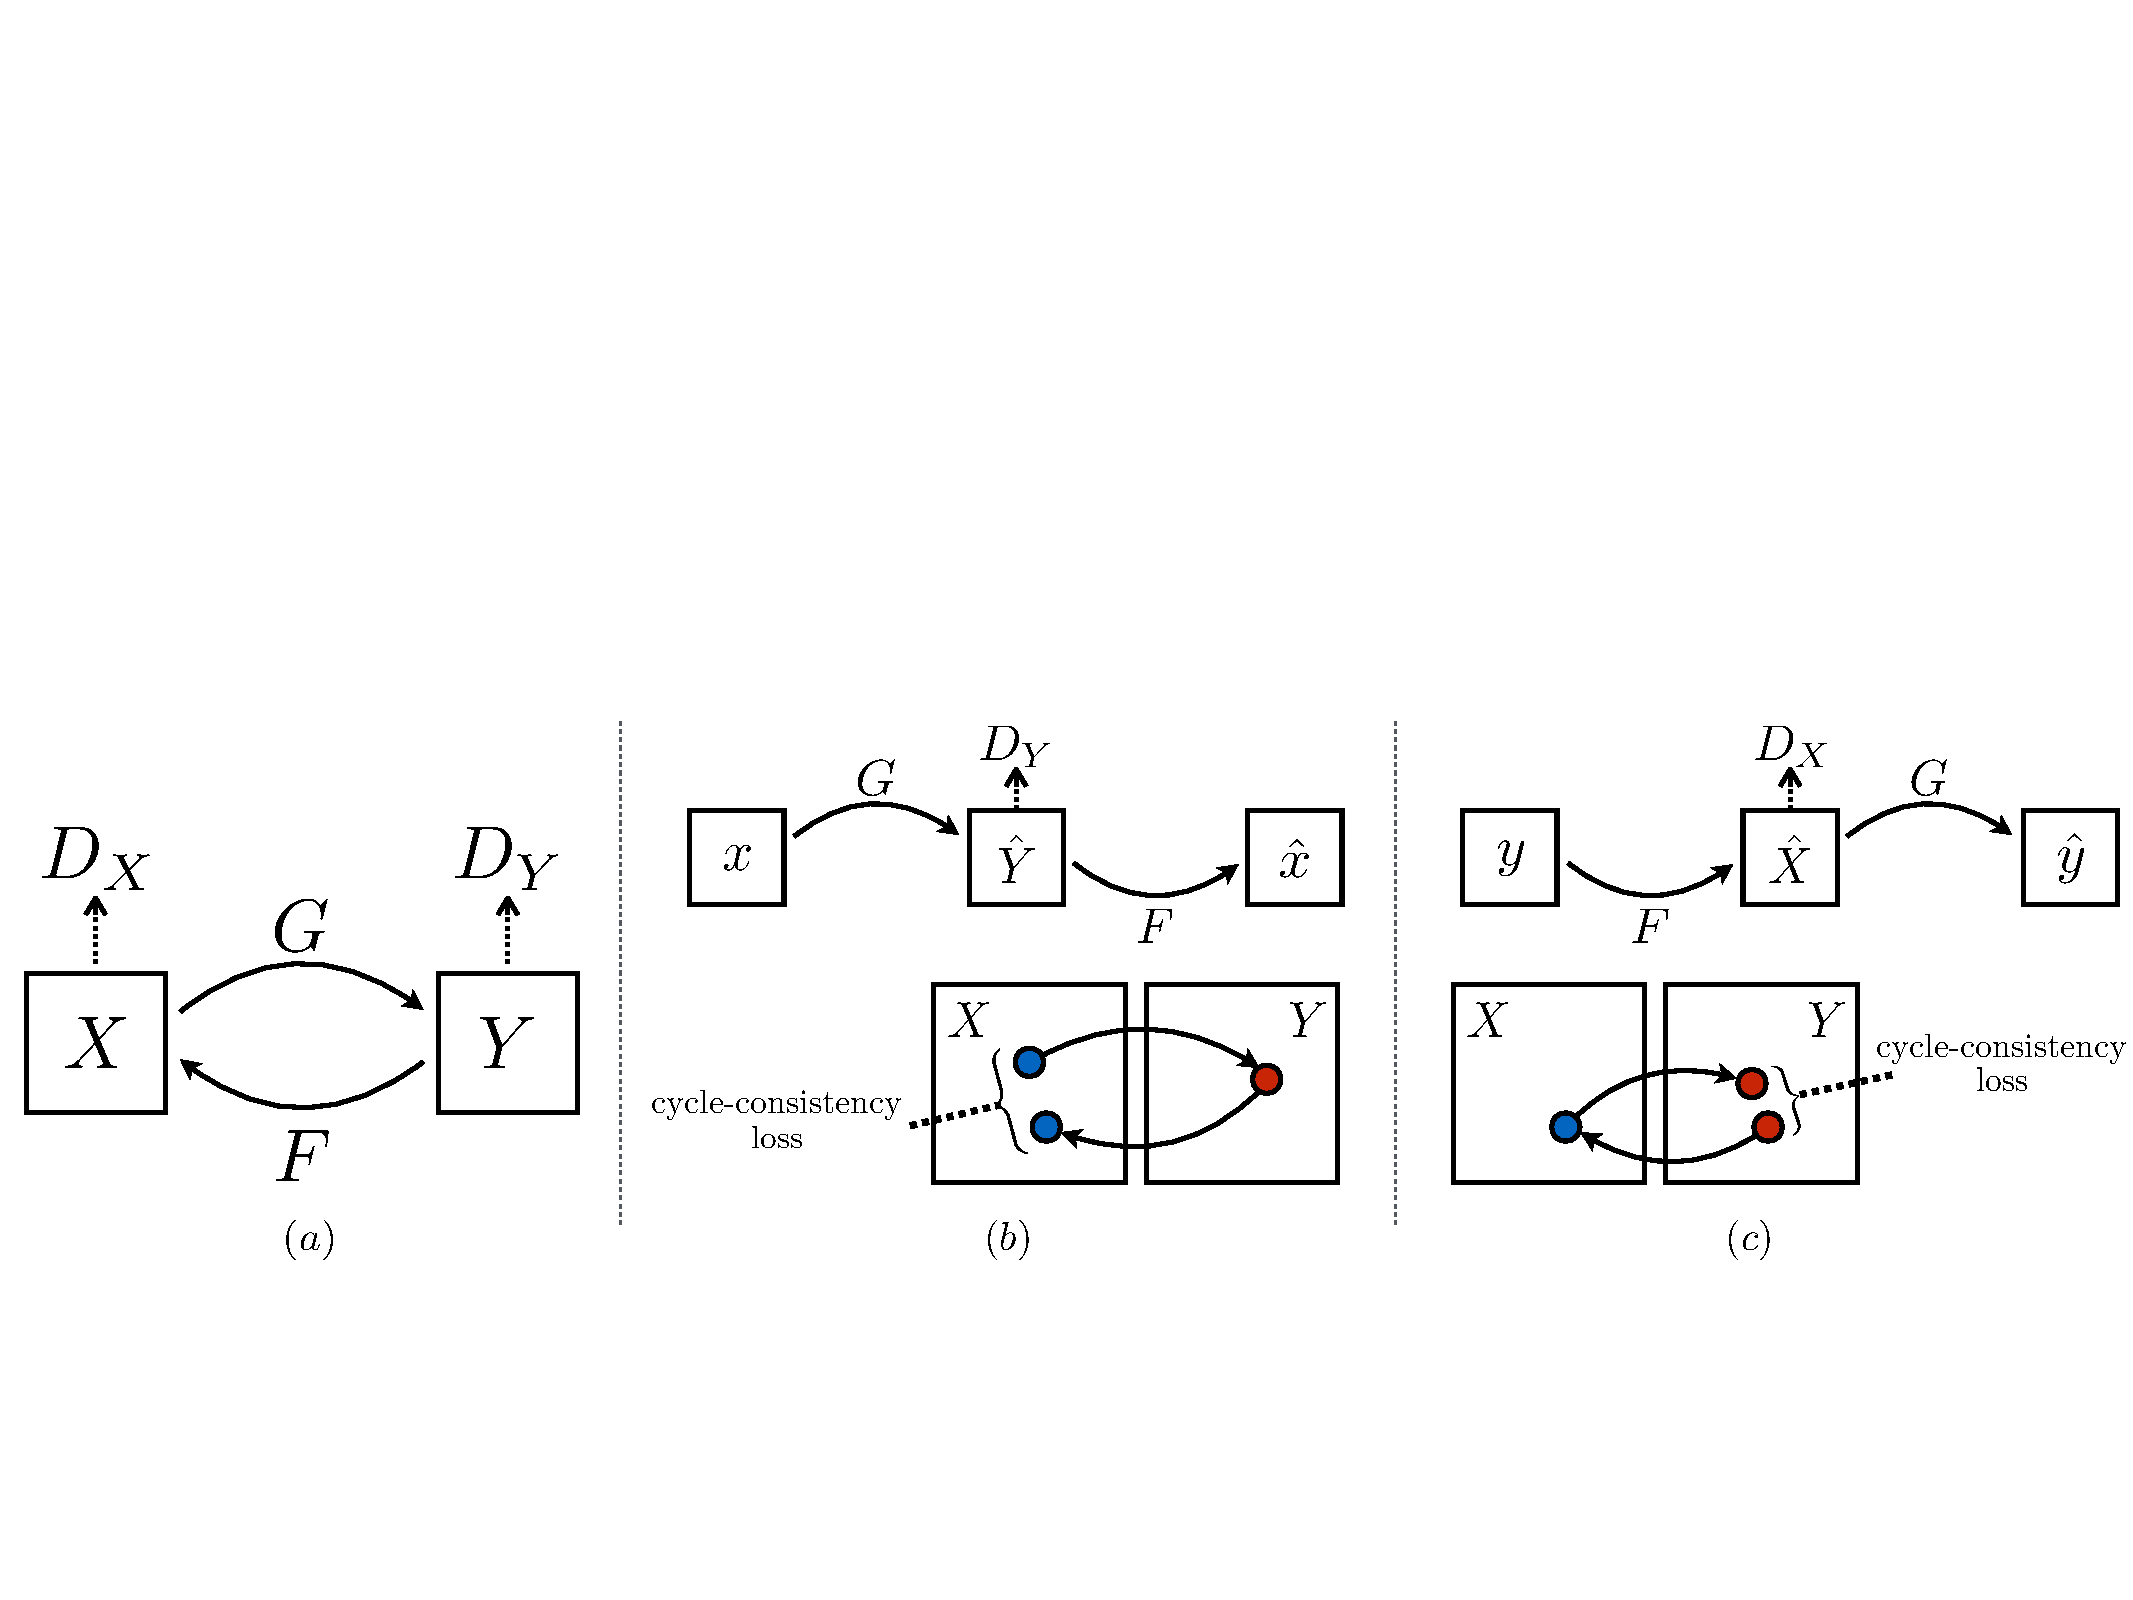
\includegraphics[width=\textwidth]{images/cycle-consistency}
	\imgsrc{\cite{zhu2017unpaired}}
	\caption{\label{fig:cycle-consistency} Cycle Consistency Loss}
\end{figure}

This training routine could also be used as an evaluation metric for other domain adaptation tasks, like text attribute style transfer. The advantage of using a cycle consistency loss is that no other content preservation metric is needed, and no domain or style specific lexicons would be needed.

In the case of our model, assume that, for a sample sentence $x$ from the domain $X$ and the ideal equivalent sentence transferred to the domain $Y$ is $y$. The transferred sentence generated by our model is $\hat{y}$. In the above approaches we compare $\hat{y}$ with the original $x$ using a content similarity metric. However, if the cycle consistency loss were to be used, we can further transfer the style of the sentence $\hat{y}$ back to the domain $X$, obtaining $\hat{x}$. Now that we have two sentences in the same domain $x$ and $\hat{x}$, it is a lot simpler to compare them, and this can be achieved by traditional parallel corpora evaluation metrics like BLEU \citep{papineni2002bleu}.

However, in our problem, assuming a scenario in which both functions $F$ and $G$ do not successfully disentangle style and content, and transfer a content as well as style at inference time, like the examples presented in \ref{tab:poor-content-preservation}. In this case, the transformation could look like
\begin{equation*}
	x \xrightarrow{G} y^* \xrightarrow{F} x
\end{equation*}
where $y^*$ is a sentence with the requisite transferred style, as well as undesirable transferred content. Such examples would score highly on both the style transfer strength metric and the cycle consistency metric.

Hence, metric would not be able to tell the difference between a model with poor content preservation and a good model, and we refrain from using it in our evaluation.


\section{Experiment Results}

\subsection{Disentangling Latent Space}

We first analyse how the style (sentiment) and content of the latent space are disentangled. We train a softmax classifier from each latent space, style and content, alongside our autoencoder model and train it to predict the true class of an input sample. The results are shown in Table \ref{tab:latent-space-classification}. vae-The results reported here are for the Yelp dataset.

In our experiments, we use an 8-neuron layer for the style embedding and a 128-neuron layer for the content embedding. We see that the 128-dimensional content vector is not discriminative for style. It achieves a classification accuracy that is slightly better than random/majority guess. However, the 8-dimensional style vector $\bm s$, despite its low dimensionality, achieves significantly higher style classification accuracy. When combining content and style vectors, we achieve no further improvement. These results verify the effectiveness of our disentangling approach, because the content space doesn't contain style information, opposed to the style space.

\begin{table}[ht]
	\centering
	\begin{tabular}{| l | r | r |}
		\hline
		                                        & \textbf{Deterministic} & \textbf{Variational} \\
		\hline \hline
		Random/Majority guess                   & 0.6018                 & 0.6018               \\ \hline \hline
		Content latent space  ($\bm c$)         & 0.6137                 & 0.6567               \\ \hline
		Style latent space ($\bm s$)            & 0.7927                 & 0.7911               \\ \hline
		Complete latent space ($[\bm s;\bm c]$) & 0.7918                 & 0.7918               \\
		\hline
	\end{tabular}
	\caption{Style classification accuracy}
	\label{tab:latent-space-classification}
\end{table}


The latent space can also be visualized with our method since we are able to infer a pair of style and content embeddings for every training data sample. We use t-SNE plots \cite{maaten2008visualizing} and use a random sample from each label to plot both the style and content embeddings inferred for them during a given epoch of the training procedure. Our hypothesis is that while the points for different labels plotted in the content embedding space would be mixed and indistinguishable in terms of plot co-ordinates, the style embedding space would display the opposite characteristic and show a clean separation of samples from each label.

We T-SNE show plots of both and deterministic autoencoder (DAE) and variational autoencoder (VAE) models in Figure \ref{fig:dae-tsne} and Figure \ref{fig:vae-tsne}, respectively.

\begin{figure}[ht]
	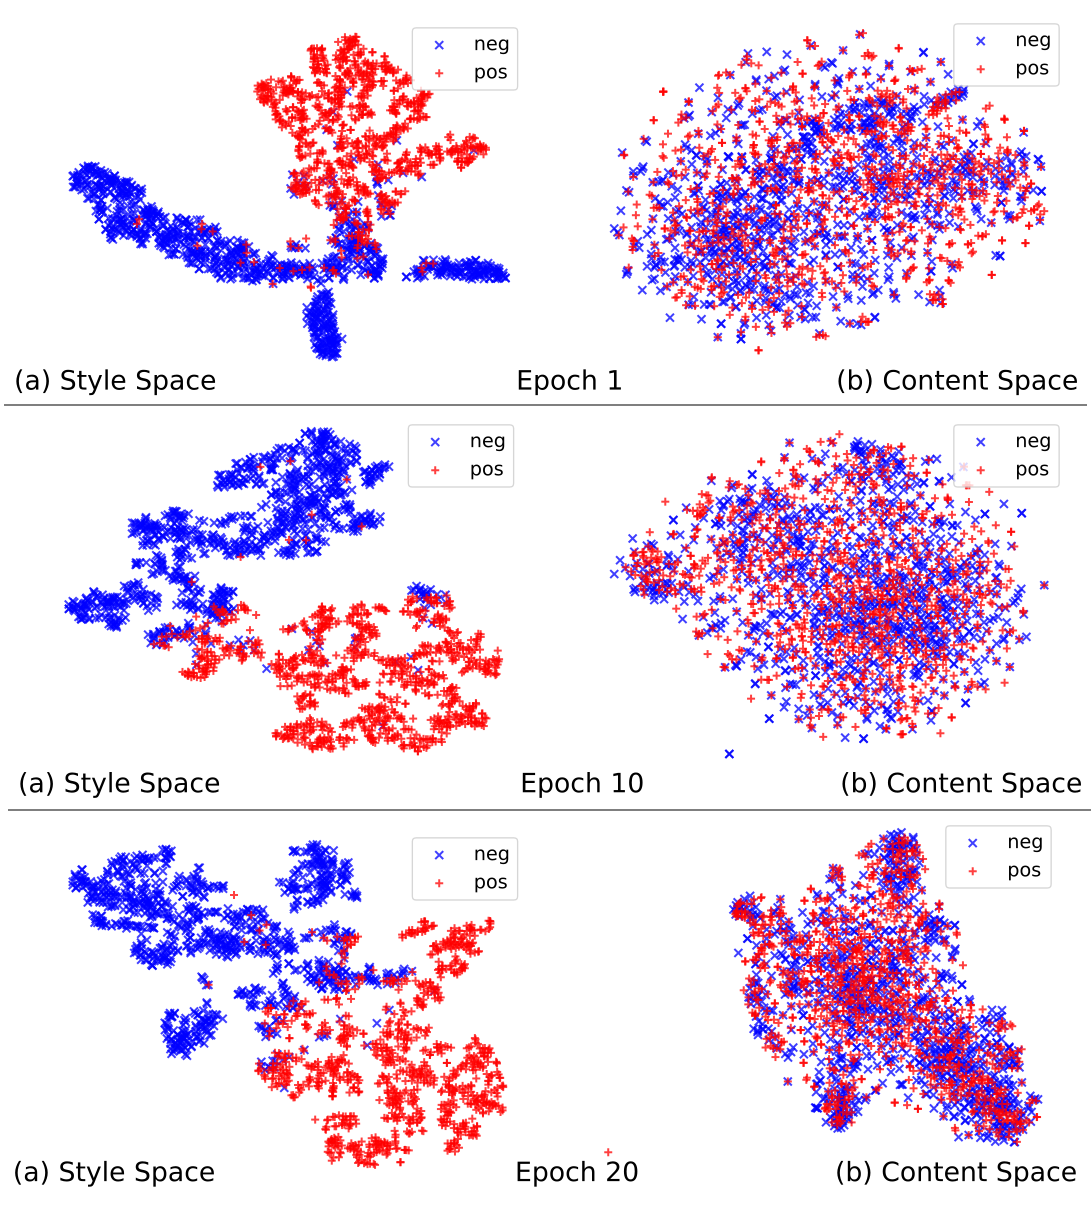
\includegraphics[width=\linewidth]{images/dae-latent-spaces}
	\caption{t-SNE plots of (a) style and (b) content spaces in the DAE model}
	\label{fig:dae-tsne}
\end{figure}

\begin{figure}[ht]
	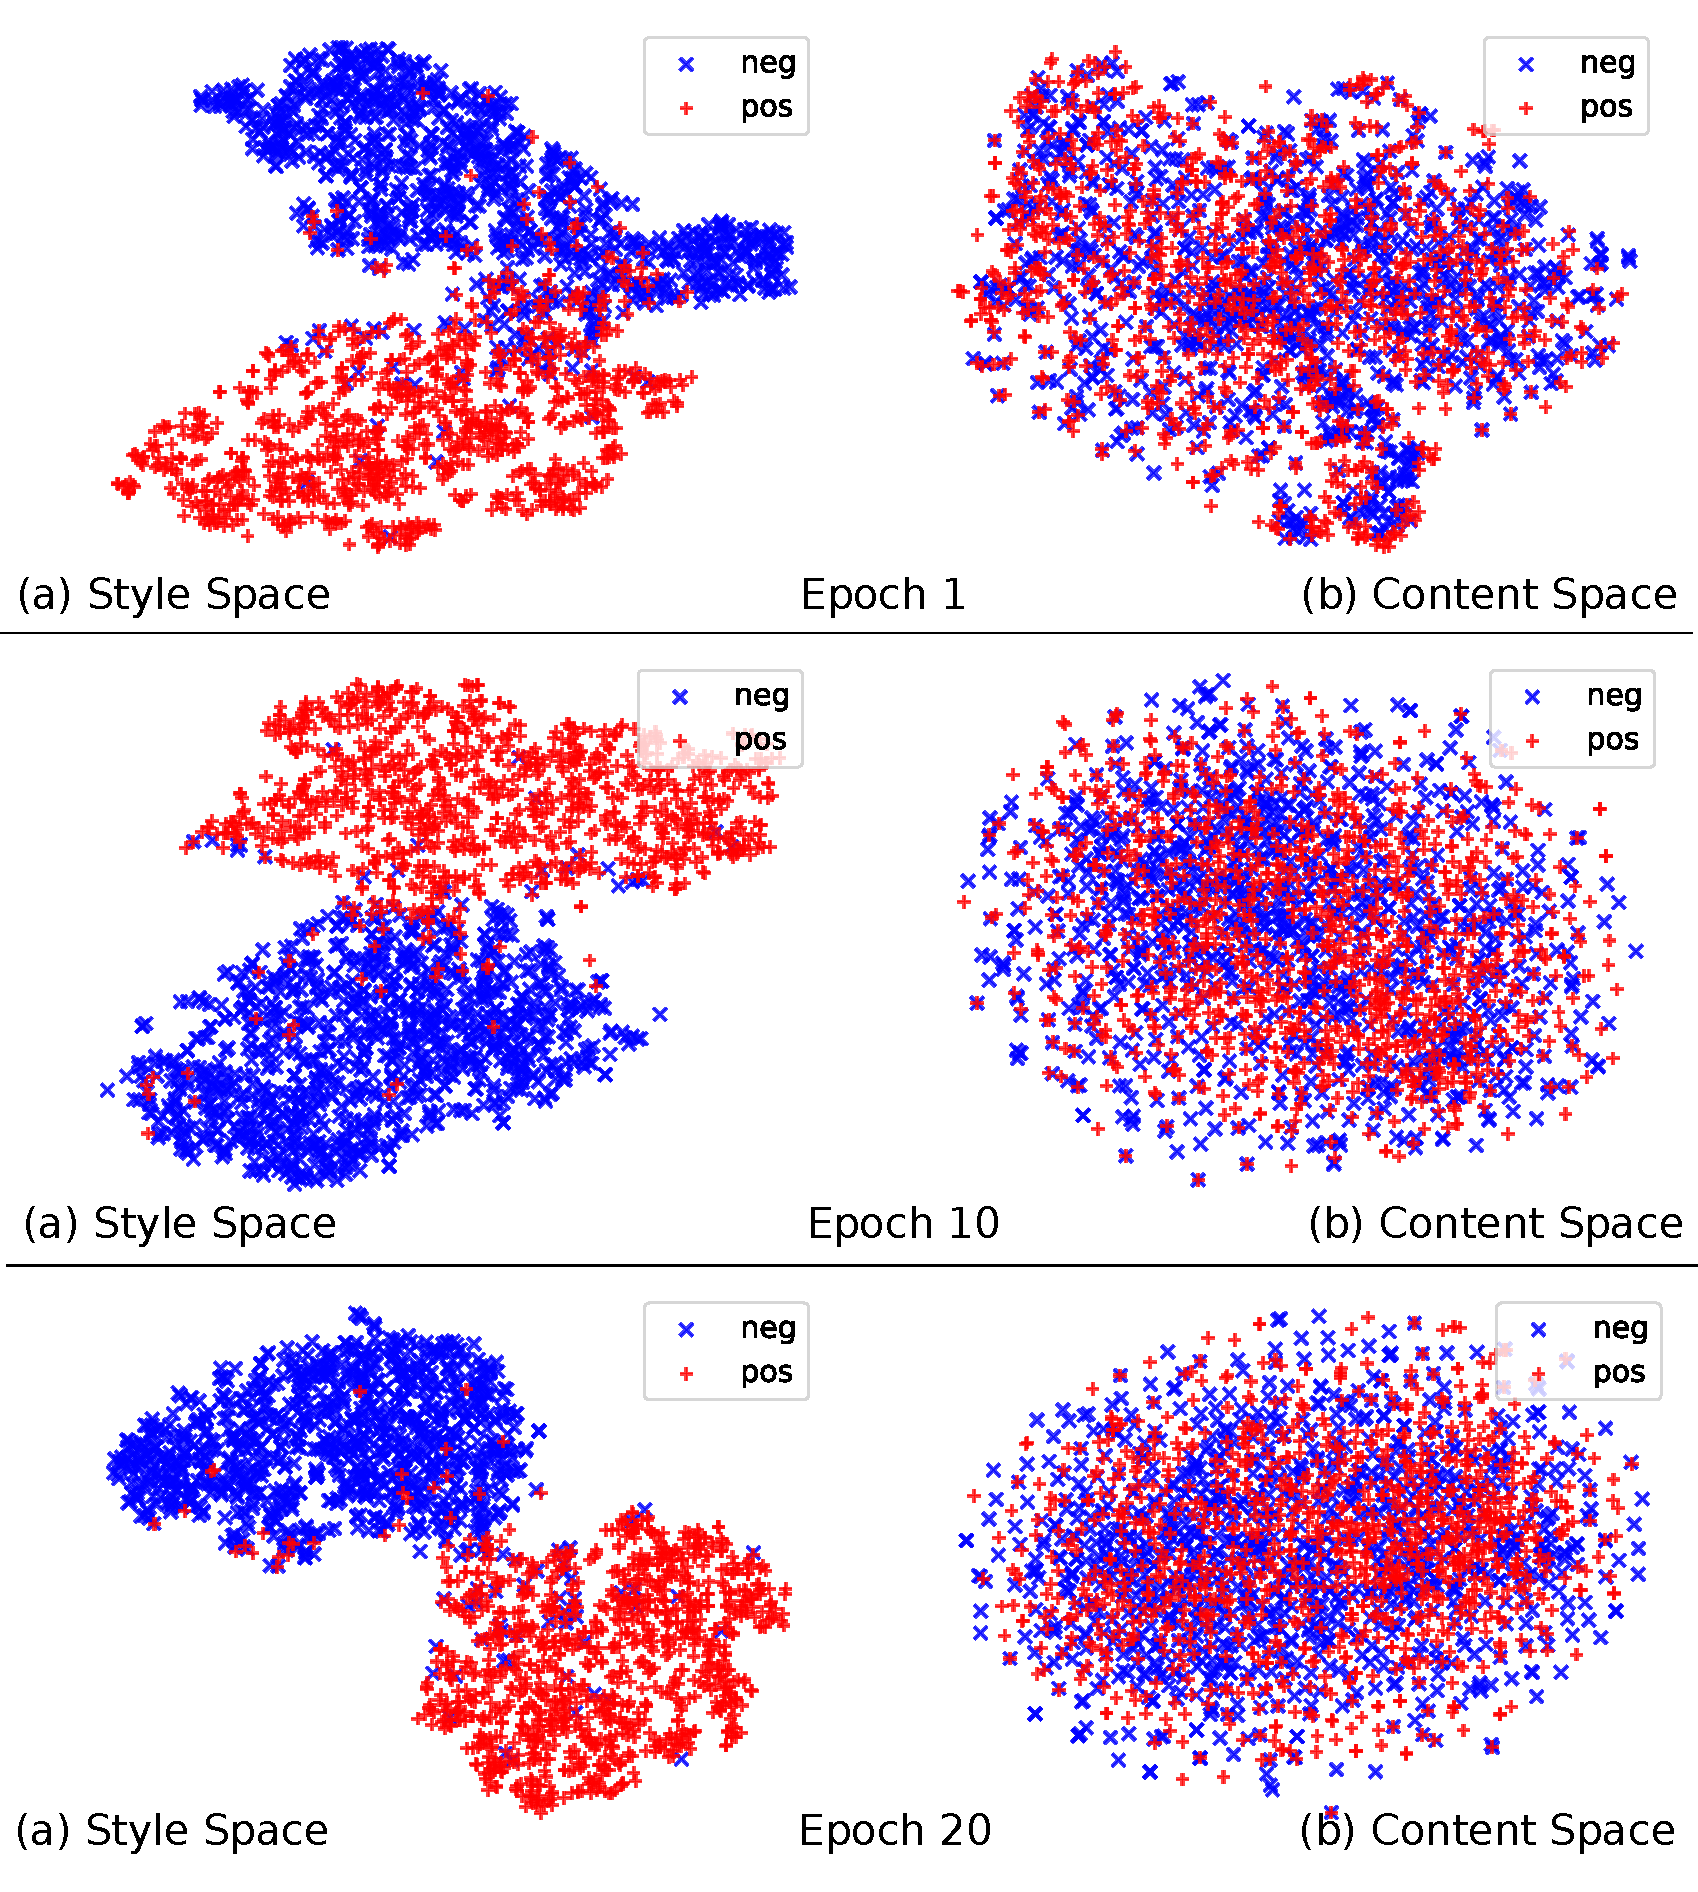
\includegraphics[width=\linewidth]{images/vae-latent-spaces}
	\caption{t-SNE plots of (a) style and (b) content spaces in the VAE model}
	\label{fig:vae-tsne}
\end{figure}

As can be seen from the plots, sentences with different styles are noticeably separated in a cleaner manner in the style space (LHS), but are indistinguishable in the content space (RHS). It is also evident that the latent space learned by the variational autoencoder is significantly smoother and continuous than the one learned by the deterministic autoencoder. Since we are essentially given the decoder a previously unseen combination of style and latent space at inference time, our hypothesis is that using a variational autoencoder would lead to more fluent generated sentences.


\subsection{Style-Transferred Text Generation}

We apply the disentangled latent space to a style-transfer sentence generation task, where the goal is to generate a sentence with different sentiment (style). We use the metrics discussed in \ref{sec:evaluation-metrics} to evaluate our models.

We compare our approach with state-of-the-art previous work in Table \ref{tab:comparison-previous}. We re-conducted the experiments with their publicly available code and data.

Results show that, our approach achieves a comparable content-preservation score to previous work, but a significantly better style-transfer score, showing that our disentangled latent space can be used for better style-transfer sentence generation.

\begin{table}[ht]
	\centering
	\begin{tabular}{| l | r | r | r |}
		\hline
		\multirow{2}{*}{
		\textbf{Model}}                       & \textbf{Style}    & \textbf{Content}      & \textbf{Word}    \\
		                                      & \textbf{Transfer} & \textbf{Preservation} & \textbf{Overlap} \\
		\hline
		\hline
		Cross-alignment \citep{shen2017style} & 0.8086            & 0.8919                & 0.2086           \\
		\hline
		Style Embedding \citep{fu2017style}   & 0.1819            & 0.9585                & 0.6661           \\
		\hline
		Ours (DAE)                            & 0.8425            & 0.8924                & 0.2551           \\
		Ours (VAE)                            & 0.8903            & 0.8824                & 0.2105           \\
		\hline
	\end{tabular}
	\caption{Comparison with previous approaches on the Yelp Dataset}
	\label{tab:comparison-previous}
\end{table}


Table \ref{tab:ablation-results} presents the results of an ablation test. We see that both, the adversarial loss and multi-task losses, play a role in the strength of style transfer. It also shows that their usage in a combination can further boost performance of the style-transfer strength.

\todo[inline]{Update ablation tests table with latest results}

\begin{table}[ht]
	\centering
	\begin{tabular}{| l | r | r |}
		\hline
		\textbf{Training Objectives}                                                  & \textbf{Style Transfer} & \textbf{Content Preservation} \\
		\hline
		\hline
		$\mathcal{L}_\text{rec}$                                                      & 0.5053                  & 0.9103                        \\
		\hline
		$\mathcal{L}_\text{rec}$, $\mathcal{L}_\text{adv}$                            & 0.5901                  & 0.9121                        \\
		\hline
		$\mathcal{L}_\text{rec}$, $\mathcal{L}_\text{mult}$                           & 0.6445                  & 0.9053                        \\
		\hline
		$\mathcal{L}_\text{rec}$, $\mathcal{L}_\text{adv}$, $\mathcal{L}_\text{mult}$ & 0.7708                  & 0.8958                        \\
		\hline
	\end{tabular}
	\caption{Ablation test.}
	\label{tab:ablation-results}
\end{table}

Some examples of style-transfer sentence generation are illustrated in Table \ref{tab:transfer-samples}. We see that, with the empirically estimated style vector, we can flexibly control the sentiment of generated sentences.

\todo[inline]{Update text samples table with latest results}

\begin{table}[ht]
	\centering
	\begin{tabular}{| p{0.45\linewidth} | p{0.45\linewidth} |}
		\hline
		\textbf{{Original}}                                                        & \textbf{Transferred (Positive $\rightarrow$ Negative)}                    \\
		\hline
		\hline
		i bought this cuisipro mister to replace my old mister last june-(number)  & i bought this a couple of times and was disappointed in this product      \\
		\hline
		quality is good, recevied in time and works as expected.                   & quality is good but i am returning it                                     \\
		\hline
		all in all, i am very happy with this headset.                             & all in all i was expecting a good product                                 \\
		\hline
		\hline
		\textbf{{Original}}                                                        & \textbf{Transferred (Negative $\rightarrow$ Positive)}                    \\
		\hline
		\hline
		i sent it back and requested a refund, and never got the refund.           & i sent it back and gave it a try and it works great                       \\
		\hline
		so i tried just one (number) piece each n still the same results.          & so i bought the two sizes and the other ones are great                    \\
		\hline
		i am going to buy a replacement and wish i had sent this back for a refund & i am going to go through the same time and i have been using it for years \\
		\hline
	\end{tabular}
	\caption{Examples of style-transfer generation.}
	\label{tab:transfer-samples}
\end{table}


%======================================================================
\chapter{Conclusion and Future Work}
%======================================================================

\section{Summary}

In this thesis, we have presented a model that utilizes previously proposed representation learning objectives like multi-task classification and adversarial learning to disentangle the latent space of a language model. We also propose a novel multi-adversary setup using a bag-of-words classification objective. We empirically show the successful disentanglement of the latent spaces, both by using auxiliary classification objectives on the learned latent spaces, and also by visualizing empirical samples using t-SNE plots.

We show that the model maintains a balance between style transfer strength and content preservation, and outperforms state-of-the-art models with respect to the style transfer strength, while performing comparably on content preservation and word overlap. In terms of fluency as measured by the Kneser-Ney language model, our variational autoencoder model outperforms all other models, while simultaneously obtaining significantly better style transfer strength scores. The deterministic autoencoder model performs slightly worse in terms of style transfer strength and fluency, but still eclipses the previous state-of-the-art, in terms of style transfer strength, content preservation and word overlap. We also quantitatively demonstrate that the addition of each of the training objectives we propose individually improves the style transfer strength capabilities of the model.

We open-source our implementation under a permissive license \footnote{\url{https://github.com/vineetjohn/linguistic-style-transfer}} so that the general framework can be applied to other problems that are thematically similar, and can be re-purposed for extensions to the model, described below.


\section{Future Direction}

\subsection{Model Improvements}

Albeit effective at the task it sets out to do, there are several improvements to the model that could be evaluated to improve its efficacy, including:
\begin{itemize}
	\item Unsupervisedly building a lexicon based on word association with each label from the training corpora, such that a hand-crafted lexicon like \cite{hu2004mining} for sentiment is not needed during evaluation.
	\item The existing model supports transfer between an arbitrary number of discrete labels. However, it can also be easily extended, by training a regressor in place of a classifier, to continuous labels. For instance, ratings on a scale from 1-5 in Amazon/Yelp reviews, controlling generation on a continuous scale for emotion valence etc.
	\item Although the adversarial learning process is quite effective in the current model, many others have found the adversarial objective hard to train because the family of $f$-divergences tend to max-out and provide no meaningful gradients. Using an optimal transport metric like the Wasserstein-1 (Earth Mover's Distance) metric seems to address this problem and stabilize training \citep{arjovsky2017wasserstein, gulrajani2017improved}. This could improve the content space disentanglement of our model.
	\item Since a variational autoencoder is hard to train due to the requirement of manually crafting KL divergence annealing procedures, an alternative is to use a Wasserstein autoencoder \citep{tolstikhin2017wasserstein}, that uses empirical sampling from the encoded distribution and a Gaussian distribution, and can effectively replace the KL divergence objective for VAEs.
\end{itemize}


\subsection{Other Domains of Application}

Although this thesis focuses attention mainly on sentiment transfer as a proxy for general style transfer, this model can also be  rely on modifications of latent attributes in text, like controlling the style of an author or an artist, modelling other attributes like generated sentence length. Discourse style could also be modelled and controlled by changing the autoencoder framework to an encoder-decoder framework.


%----------------------------------------------------------------------
% END MATERIAL
%----------------------------------------------------------------------

% B I B L I O G R A P H Y
% -----------------------

% The following statement selects the style to use for references.  It controls the sort order of the entries in the bibliography and also the formatting for the in-text labels.
\bibliographystyle{unsrtnat}
% This specifies the location of the file containing the bibliographic information.  
% It assumes you're using BibTeX (if not, why not?).
\cleardoublepage % This is needed if the book class is used, to place the anchor in the correct page,
% because the bibliography will start on its own page.
% Use \clearpage instead if the document class uses the "oneside" argument
\phantomsection  % With hyperref package, enables hyperlinking from the table of contents to bibliography             
% The following statement causes the title "References" to be used for the bibliography section:
\renewcommand*{\bibname}{References}

% Add the References to the Table of Contents
\addcontentsline{toc}{chapter}{\textbf{References}}

\bibliography{uw-ethesis}
% Tip 5: You can create multiple .bib files to organize your references. 
% Just list them all in the \bibliogaphy command, separated by commas (no spaces).

% The following statement causes the specified references to be added to the bibliography% even if they were not 
% cited in the text. The asterisk is a wildcard that causes all entries in the bibliographic database to be included (optional).
\nocite{*}

\end{document}
